%  PARA TRABALLOS EN GALLEGO USAR (LINEA 12): \usepackage[galician]{babel}
%  PARA TRABALLOS EN CASTELLANO USAR (LINEA 13): \usepackage[spanish]{babel}
%
% Para los acentos usamos codificacion UTF-8 (LINEA 10): \usepackage[utf8]{inputenc} 
% Si se usase la codificacion es_ES.ISO-8859-1 (LINEA 11): \usepackage[latin1]{inputenc}
% La conversion de acentos se hace con: iconv -f UTF-8 -t ISO-8859-1 filename.tex
%
% Como se incluyen figuras eps hay que compilar con: latex traballo , dvipdf traballo
%

\documentclass[12pt,twoside,a4paper]{book}
% pódense engadir todos os packages necesarios
\usepackage[utf8]{inputenc}
% \usepackage[latin1]{inputenc}
%\usepackage[galician]{babel}
\usepackage[spanish]{babel}
\usepackage{graphicx}
\usepackage[dvips]{epsfig}
\usepackage{amssymb}
\usepackage{eurosym}
\usepackage{float}
\usepackage{latexsym}
\usepackage{a4}
\usepackage{listings}
\usepackage{multirow}
\usepackage[hidelinks]{hyperref} % menús no pdf pero non leva ben co package galician
\usepackage{url}
\usepackage{rotating}
\usepackage{caption}
\usepackage[section]{placeins}
\usepackage{booktabs}
\usepackage{tabularx} % Better tables
\usepackage{enumitem}
\usepackage{xcolor}
\usepackage{xstring, xifthen}
\usepackage[nottoc, notlot, notlof, notindex]{tocbibind}

%%% Datos del TFG
\newcommand{\tfgauthor}{Rub{\'e}n Mosquera Varela}
\newcommand{\tfgtutor}{Jos{\'e} Ram{\'o}n R{\'i}os Viqueira}
\newcommand{\tfgcotutor}{Manuel Antonio Regueiro Seoane}
\newcommand{\tfgtitle}{Visualización de observacións en SIX de escritorio}
\newcommand{\tfgsubtitle}{}
\newcommand{\tfgtitleshort}{Memoria SOS Client} %Para meta-datos PDF
\newcommand{\tfgcopyright}{Copyright (C) 2015, \tfgauthor}
\newcommand{\tfglicense}{Creative Commons (by-sa) 2.5 Spain}
\newcommand{\tfglicenseurl}{http://creativecommons.org/licenses/by-sa/3.0/}
\newcommand{\tfgkeywords}{TODO}
\newcommand{\logoUni}{images/logo_usc.eps} % Logotipo de la Universidad

%%%
% CONFIG: Meta-datos para inclusión en PDF y XMP
%
\hypersetup{
    pdftitle        = {\tfgtitleshort},
    pdfauthor       = {\tfgauthor},
    pdfsubject      = {\tfgtitle},
    pdfkeywords     = {\tfgkeywords},
    pdfcreator      = {\tfgauthor},
    pdfproducer     = {\tfgauthor~powered~by~\LaTeX},
    pdfcopyright    = {\tfgcopyright},
    pdflicenseurl   = {\tfglicenseurl},
    pdfstartview    = FitB                      % Ajustar la página a la ventana
}

%----------------------------------------------------------------------------------------
%	FLOATS: TABLES, FIGURES AND CAPTIONS SETUP
%----------------------------------------------------------------------------------------
\usepackage{booktabs}
\usepackage{tabularx} % Better tables
\setlength{\extrarowheight}{3pt} % Increase table row height
%\newcommand{\tableheadline}[1]{\multicolumn{2}{c}{#1}}
\newcommand{\risktable}[7]{
	\begin{table}[H]
	\centering
		\begin{tabularx}{\textwidth}{lXl} \toprule
		\multicolumn{2}{l}{{#1}.-{#2}} \\
		\cmidrule(r){1-2}
		\textbf{Descrición} &  #3\\ 
		\textbf{Probabilidade} &  #4\\ 
		\textbf{Impacto} &  #5\\ 
		\textbf{Nivel de exposición} &  #6\\ 
		\textbf{Resposta ao risco} &  #7\\ 
		\bottomrule
		\end{tabularx}
	\caption{{#1}.-{#2}}
	\label{tab:#1}
	\end{table}}

%----------------------------------------------------------------------------------------
%	HYPHENATION
%----------------------------------------------------------------------------------------
\hyphenation{In-te-re-se}
\hyphenation{CiTIUS}
\includeonly{capitulos/titulo,capitulos/certificacion,capitulos/xestiondoproxecto,capitulos/analise}
%\includeonly{capitulos/analise}
\begin{document}
%%Se reeditan estas funciones para sacar el texto en gallego usando el idioma spanish, porque galician no funciona con hyperref
\renewcommand{\contentsname}{Índice xeral}
\renewcommand{\listtablename}{Índice de cadros}
\renewcommand{\tablename}{Cadro} 
\pagestyle{empty}
\begin{center}
{\bf\Large UNIVERSIDADE DE SANTIAGO DE COMPOSTELA}

\vspace{0.5cm}
\includegraphics[width=5cm]{\logoUni}

\vspace{0.5cm}
{\bf\large ESCOLA TÉCNICA SUPERIOR DE ENXEÑARÍA}

\vspace{2cm}
{\bf\LARGE \tfgtitle}

\vspace{0.5cm}
{\bf\LARGE \tfgsubtitle}
\end{center}

\vspace{2cm}
\hspace{4cm}\begin{tabular}{l}
{\it\Large Autor:} \\
{\bf\Large \tfgauthor} \\
~ \\
{\it\Large Directores:} \\
{\bf\Large \tfgtutor} \\
{\bf\Large \tfgcotutor} \\
\end{tabular}

\vspace{2cm}
\begin{center}
{\bf\Large Grao en Enxeñaría Informática}

\vspace{0.5cm}
{\bf\large Xullo 2015}

\vspace{0.5cm}
Traballo de Fin de Grao presentado na Escola Técnica Superior de Enxeñaría da Universidade de Santiago de Compostela para a obtención do Grao en Enxeñaría Informática
\end{center}


\cleardoublepage
\pagestyle{plain}
\pagenumbering{roman}

\includegraphics[width=4cm]{images/logo_usc.eps}

\vspace{1cm}
{\bf D. \tfgtutor}, Profesor do Departamento de Electrónica e Computación da Universidade de Santiago de Compostela, e {\bf D. \tfgcotutor}, TODO poñer aquó o cargo,

\vspace{1cm}
INFORMAN:

\vspace{1cm}
Que a presente memoria, titulada {\it \tfgtitle}, presentada por {\bf D. \tfgauthor} para superar os créditos correspondentes ao Traballo de Fin de Grao da titulación de Grao en Enxeñaría Informática, realizouse baixo nosa dirección no Departamento de Electrónica e Computación da Universidade de Santiago de Compostela.

\vspace{1cm}
E para que así conste aos efectos oportunos, expiden o presente informe en Santiago de Compostela, a 10 de Xullo de 2015:

\vspace{2cm}
\begin{tabular}{lll}
O titor, & O cotitor, & O alumno, \\
~ \\
~ \\
~ \\
~ \\
~ \\
~ \\
~ \\
\tfgtutor & \tfgcotutor & \tfgauthor
\end{tabular}

 % paxina de certificación (optativa)
%\cleardoublepage
%\pagestyle{plain}
\chapter*{Agradecementos}
A Olatz, pola motivación, o ánimo e o apoio. % paxina de agradecementos (optativa) 
\cleardoublepage
\pagestyle{plain}
\chapter*{Resumo}
Aquí vai o resumo

 % páxina de resumo (optativa) 

\cleardoublepage
\pagestyle{plain}
\tableofcontents
\listoffigures
\listoftables

% Agora incluimos os capítulos. Cambiamos a numeración e as cabeceiras
\cleardoublepage
\pagenumbering{arabic}
\setcounter{page}{1}
\pagestyle{headings}
\chapter{Introdución}
\section{Contextualización}
Dende sempre o ser humano tivo inquietude por coñecer e entender como funciona o medio que nos rodea, tarefa para a que resulta imprescindible a observación do mesmo. A observación defínese como a captación activa e rexistro de información dende unha fonte primaria, a través dos sentidos ou da utilización de instrumentos.

Dada o crecente interese polo estado do medio ambiente e os avances tecnolóxicos que se produciron nas últimas décadas, na actualidade xérase a cada instante unha inxente cantidades de datos que rexistran medicións dunha ampla variedade de fenómenos, empregando para elo os máis diversos métodos, dende modernos sensores montados satélites ata o rexistro manual das medicións realizadas por un sinxelo termómetro de mercurio.

As maiores dificultades para converter este gran volume de datos en información útil son debidas a heteroxeneidade dos mesmos, tanto pola súa natureza física como polos medios empregados para capturalos e rexistralos.

Para atallar este problema xurdiu dende o Open Geospatial Consortium\footnote{\url{http://www.opengeospatial.org/}} (OGC) a iniciativa de desenvolver un estándar, denominado Sensor Observation Service (SOS), que defina un modelo interoperable para a difusión a través de servizos web de calquera tipo de información relacionada con sensores, do tipo que sexan.

O OGC\footnote{Que é o OGC? - \url{https://www.youtube.com/watch?v=bfkCdir-yO8}} é un consorcio formado por empresas privadas, universidades e axencias gobernamentais de todo o mundo, co obxectivo de desenvolver e publicar estándares no eido da información xeoespacial. É a organización de referencia neste eido, fundada no 1994 conta na actualidade con máis de cincocentos membros e continúa medrando.

O estándar SOS define a interface do servizo web que permite consultar observacións, metadatos dos sensores e a representación das entidades observadas. Amais define os medios para rexistrar novos sensores ou eliminar os existentes, así como para inserir novas observacións para os sensores. Este estándar apoiase en outros, tamén desenvolvidos polo OGC, que definen os modelos para a representación dos datos a comunicar, así pois as xeometrías das entidades observadas represéntase a través do Geography Markup Language (GML), os metadatos dos sensores a través do SensorML e as observacións a través do estándar Observations and Measurements (O\&M).

As observacións de fenómenos medio ambientais son pois un tipo de información xeográfica, de feito tan importante coma a medición realizada do fenómeno a observar son o lugar o e momento no que se realiza. Pódese abordar, polo tanto, a análise e explotación destes datos empregando como ferramenta un Sistema de Información Xeográfica (SIX) de escritorio.

O acrónimo SIX fai referencia a un sistema deseñado para capturar, almacenar, manipular, analizar e presentar calquera tipo de información xeograficamente referenciada. Dentro do software SIX distínguense varios grandes grupos segundo o seu propósito, como poden ser sistemas de xestión de bases de datos espaciais, servidores cartográficos, visores web, móviles ou de escritorio. Dentro deste último grupo, os SIX de escritorio, inclúense un amplo número de programas que permiten visualizar, editar e analizar datos xeográficos e que se empregan en moitos eidos e con moi diversos fins, por exemplo para investigacións científicas, meteoroloxía, cartografía, hidroloxía, xestión de recursos, marketing, loxística, avaliación do impacto ambiental, etc.

Os SIX traballan principalmente con dous formatos de información, segundo os obxectos do mundo real que se vaian representar sexan de natureza continua ou discreta. Así pois, para representar unha variable de natureza continua, como por exemplo un mapa da elevación do terreo, empregase o formato raster, que divide o espazo en celas regulares asociando un valor a cada unha delas. Pola contra, para representar obxectos de natureza discreta, como pode ser un río, emprégase xeralmente o formato vectorial, no que se representa a xeometría en base a puntos, liñas ou polígonos, e se lle asocian a esta xeometría os atributos e valores que sexan necesarios. Cabe destacar que estes dous formatos poden converterse entre si se en función da análise a realizar, por exemplo, en base as observacións de temperaturas en determinados puntos pódese xerar por interpolación un raster que represente o mapa térmico da zona (rasterización), ou pola contra, a partir dun mapa de elevación poder trazar as curvas de nivel que o representan (vectorización).

En canto as ferramentas de análise proporcionadas polos paquetes SIX, existe unha moi ampla gama técnicas que se desenvolveron principalmente no último medio século, e é un campo en cambia rapidamente na actualidade, incluíndose cada vez máis e máis ferramentas, ben proporcionadas polo propio provedor orixinal do software ou en moitos casos desenvolvidas por terceiros a través das posibilidades de ampliación que os propios programas SIX poñen a disposición dos desenvolvedores.

Na maioría dos SIX o modelado dos fenómenos xeográficos realizase de forma estática, sen embargo na actualidade requírense modelos que engadan o tempo como variable, de xeito que permitan observar o comportamento dinámico dos eventos xeográficos, como por exemplo no caso das observacións de fenómenos medio ambientais. Os SIX que incorporan a representación do tempo, amais das dimensións espaciais, denomínanse SIX temporais e permiten facer unha representación da información en 4D, o que abre un amplo abano de posibilidades. A incorporación da compoñente temporal é un dos aspectos o que máis esforzos se están a adicar no que a evolución dos SIX se refire.

\section{Motivación e Obxectivos}

Na actualidade, a area de análise e explotación da información obtida a través das observacións medio ambientais está moi fragmentada. Cada organismo ou axencia desenvolve as súas propias solucións para a captación, o almacenamento e a análise das cada vez máis amplas redes de sensores despregadas por todo o planeta. Este feito supón unha gran limitación en canto ó aproveitamento de toda esta información, o restrinxir o acceso á mesma as organizacións que dispoñen dos recursos necesarios para desenvolver e implantar os sistemas necesarios.

O estándar SOS pretende permitir a interoperabilidade entre os sistemas encargados de captar e almacenar esta información e os sistemas empregados para a análise da mesma, non obstante o grao de implantación deste estándar é aínda reducido. Como motivo, ou consecuencia, deste baixo grao de implantación existen na actualidade moi poucos sistemas de información xeográfica que inclúan o servizo SOS como unha fonte de datos soportada, a diferenza de outros estándares desenvolvidos polo OGC que son soportados pola ampla maioría dos sistemas, como o Web Map Service (WMS) ou o Web Feature Service (WFS).

As escasas solucións dispoñibles para operar con datos de observación servidos pola interface SOS en sistemas de información xeográfica pasan polo uso de extensións de terceiros para software comercial, como por exemplo ArcGIS\footnote{\url{http://www.esri.es/es/productos/arcgis/}}, que supón un elevado custe de licencia.

Este proxecto ven motivado, por tanto, pola inexistencia dun sistema de información xeográfica libre e de propósito xeral que permita a incorporación e análise de datos de observacións dispoñibles a través da interface SOS.

O obxectivo deste traballo é o desenvolvemento dunha extensión para a ferramenta SIX libre QGIS\footnote{\url{http://www.qgis.org/}} que permita a conexión a fontes de datos SOS e a exploración dos seus contidos no contorno de mapas proporcionado pola ferramenta.

\section{Entorno tecnolóxico}
\subsection{QGIS}
QGIS é un Sistema de Información Xeográfica de escritorio multiplataforma, libre e de código aberto. É un proxecto oficial da organización non gubernamental Open Source Geospatial Foundation\footnote{\url{http://www.osgeo.org/}} (OSGeo) nacido no ano 2002 co obxectivo principal de proporcionar unha ferramenta que permitise visualizar, editar e analizar datos xeográficos en calquera ordenador persoal.

Amais de proporcionar de por si soporte para un amplo número de formatos de datos e funcionalidades para operar cos mesmos, QGIS proporciona unha API completa para implementación de \emph{plugins} que amplíen a funcionalidade da ferramenta e os formatos de información xeográficos soportados. Os \emph{plugins} poden programarse en C++ ou en Python, e no caso de cumprir a normativa e ser aprobados polos responsables poden incluírse no repositorio oficial da aplicación, de xeito que se podan instalar directamente dende o propio QGIS.

QGIS é na actualidade o SIX libre de referencia, está apoiado por un gran número de organizacións que patrocinan o proxecto, e que son, xunto coas doazóns de puntuais de particulares e ou organizacións o método de financiamento do proxecto. A redor do QGIS desenvolveuse unha ampla e activa comunidade tanto de usuarios como de desenvolvedores, do propio QGIS ou de \emph{plugins}.

\subsection{Sensor Observation Service}
O estándar Sensor Observation Service\footnote{\url{http://www.opengeospatial.org/standards/sos}} define a interface do servizo web para descubrir e recuperar datos en tempo real ou arquivados producidos por calquera clase de sensor, tanto móbiles como estacionarios, in-situ ou remotos. Os datos dos sensores poden ser tanto observacións realizadas como descricións dos sensores ou metadatos dos mesmos relativos a calibracións, mantementos, etc. As observacións devólvense codificadas segundo o estándar Observations and Measurements, e a información sobre sensores a través de SensorML. O SOS define, na súa versión 1.0, tres grupos de operacións:
\begin{description}
\item[Core:] Estas operacións deben ser implementadas obrigatoriamente por todos os servizos SOS.
\begin{itemize}
\item \textit{GetCapabilities:} Esta operación é a que proporciona a descrición das capacidades do SOS, ademais de información xeral sobre o propio servizo. Entre outros datos indícanos as versións de SOS soportadas, os datos identificativos do servizo e do provedor do mesmo, as operacións que implementa (cos parámetros soportados por cada unha delas), os filtros soportados e a lista de ofertas provistas polo servizo, con información detallada de cada unha delas.
\item \textit{DescribeSensor:} Proporciona información relativa ó sensor requirido, segundo o estándar Sensor Model Language (SensorML). Entre outra información indícase a posición, nome e descrición do sensor ou sistema, o instante temporal da instalación e se proporciona medidas válidas, os fenómenos que pode medir e as unidades nas que os mide, e outra información relacionada, como un breve historial de reparacións e
calibracións, etc
\item \textit{GetObservations:} É a operación encargada de proporcionar os datos medidos polos sensores dunha determinada oferta e que cumpran os filtros definidos na consulta. Os valores destas observacións realizadas polos sensores devólvense segundo o estándar Observations and Measurements (O\&M). Este estándar define un formato de XML no que cada observación se describe polo fenómeno que mide, o sensor que o mide, o instante temporal da medida, a posición e nome do lugar no que se toma a medida e a unidade na que se mide o valor correspondente.
\end{itemize}
\item[Transactional:] Son as operacións que permiten rexistrar información no servizo. A súa implementación é opcional.
\begin{itemize}
\item \textit{RegisterSensor:} Permite rexistrar un novo sensor no servizo, mandando a súa descrición no formato SensorML.
\item \textit{InsertObservation:} Permite ó cliente inserir novas observacións no sistema de sensores que fosen previamente rexistrados.
\end{itemize}
\item[Extended:] Son operacións adicionais opcionais, para requirir información o servizo.
\end{description}

\section{Estrutura da memoria}

Este documento estrutúrase en 6 capítulos, un apéndice e a bibliografía empregada.\\

Neste capítulo de introdución descríbese a motivación e obxectivos do proxecto e contextualizase o mesmo describindo brevemente os conceptos empregados e a situación actual da técnica nas areas de coñecemento relacionadas.\\

No capítulo 2 abórdanse os aspectos relativos á xestión do proxecto: a definición do alcance, a metodoloxía, planificación temporal e xestión de riscos e da configuración.\\

No capítulo 3 detállase a análise do software, describindo os casos de uso identificados e os requisitos extraidos dos mesmos.\\

No capítulo 4 descríbese o deseño do software, tanto a arquitectura do mesmo como o comportamento de cada unha das compoñentes desde o punto de vista estático e dinámico.\\

No capítulo 5 documéntase en orde cronolóxico o proceso de implementación e as probas realizadas para cumprir os requisitos establecidos.\\

No capítulo 6 expóñense as conclusións extraidas de todo o proxecto e detállanse varias propostas de traballo futuro.\\
%\item[Apéndice A:] \textit{Manual técnico.}

O apéndice A é unha guía para a instalación e manexo básico do \emph{plugin} desenvolvido.\\
\cleardoublepage
\chapter{Xestión do proxecto}
A xestión do proxecto ten como finalidade definir e alcanzar os obxectivos do mesmo, ó tempo que se optimiza o uso de recursos, tanto humanos como materiais. Na sección III do PMBOK\cite{PMBOK} descríbense amplamente os distintos tipos de procesos que se inclúen dentro da xestión do proxecto, non obstante, para cada proxecto concreto será necesario seleccionar os máis apropiados para cumprir co obxectivo do mesmo.

\section{Alcance do proxecto}
Os procesos de xestión do alcance do proxecto son os encargados de asegurar que o proxecto inclúa o traballo requirido, e só o requirido, para completar o proxecto de forma satisfactoria.

\subsection{Definición do alcance}
O obxectivo deste proxecto é dotar ó Sistema de Información Xeográfica QGIS\footnote{http://www.qgis.org/} da capacidade de consultar fontes de datos SOS e representar os datos obtidos no contorno de mapas proporcionado pola ferramenta, de xeito que podan ser explorados e analizados polo usuario. Para acadar este obxectivo desenvolverase un engadido para o programa QGIS, coas seguintes funcionalidades:

\begin{itemize}
\item Conectarse a un servidor SOS e obter as capacidades do servizo a través da operación GetCapabilities.
\item En base as capacidades do servidor permitir xerar unha petición de observacións, de forma sinxela, sin necesidade de coñecementos técnicos do SOS.
\item Permitir modificar a petición xerada manualmente se o usuario o desexa.
\item Obter as observacións a través da operación GetObservations.
\item Coas observacións descargadas xerar unha capa vectorial que conteña a información xeográfica, temporal e os valores das propiedades observadas.
\item Xerar gráficos en dúas dimensións cos datos da capa.
\item Permitir visualizar a capa co plugin TimeManager de xeito que se podan facer animacións.
\end{itemize}

\subsection{Estrutura de Descomposición do Traballo}
A Estrutura de Descomposición do Traballo (EDT) axuda a dividir o proxecto en paquetes de traballo de forma xerárquica. Dado que se empregará a metodoloxía áxil \emph{Scrum} non é necesario detallar o EDT máis do que xa se fixo no anteproxecto, que se representa na figura \ref{fig:edt}.

\begin{figure}[hbtp]
\centering
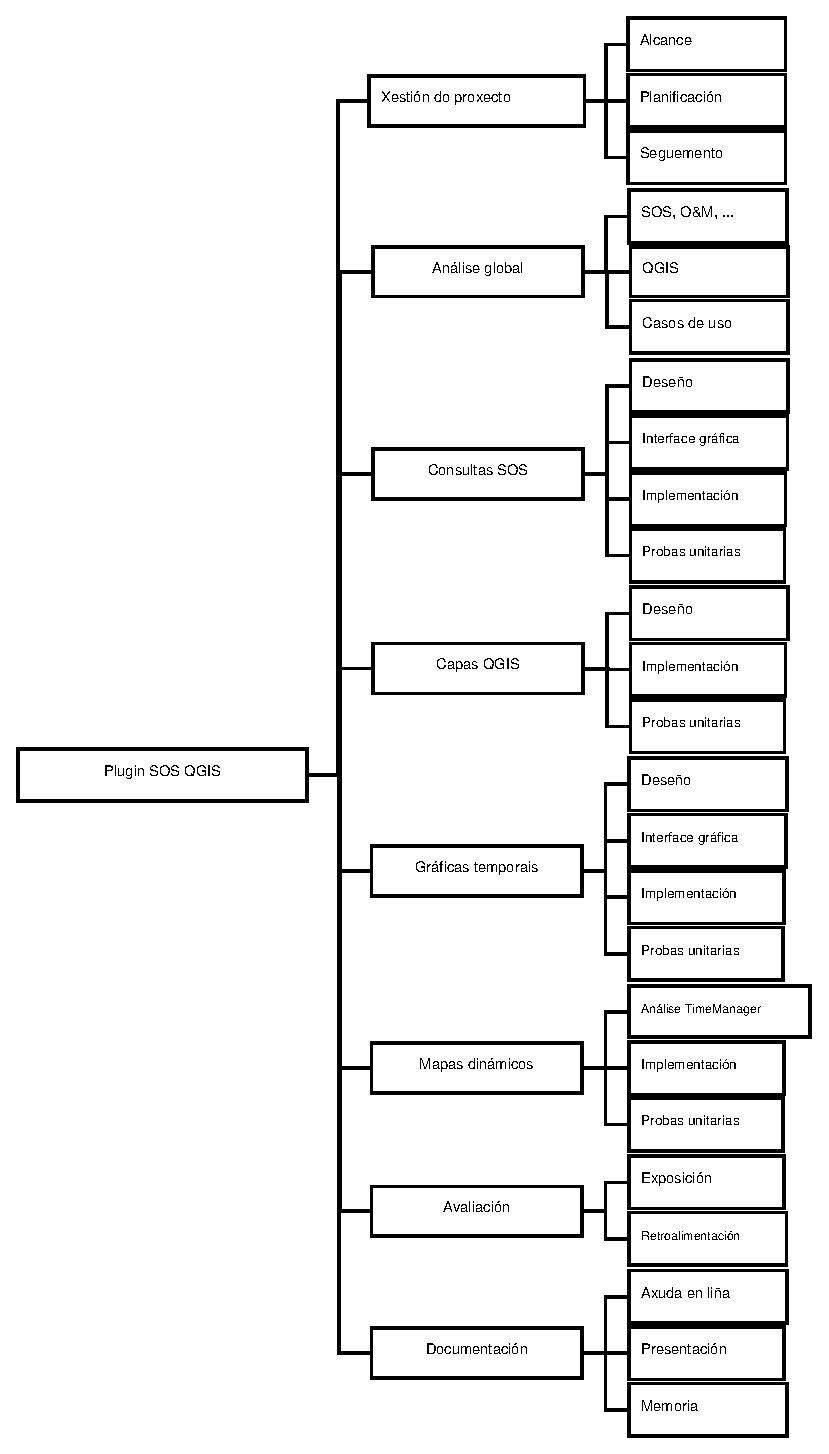
\includegraphics[scale=1]{images/edt.eps}
\caption{Estrutura de Descomposición do Traballo}
\label{fig:edt} 
\end{figure}

\section{Xestión do tempo}
A xestión do tempo do proxecto inclúe os procesos necesarios para lograr a conclusión do proxecto a tempo.

Ó empregar a metodoloxía \emph{Scrum} non se planifica inicialmente a duración de cada tarefa, non obstante si se poden identificar as distintas tarefas a levar a cabo e facer unha estimación da súa duración en base ás horas establecidas para o proxecto e a importancia de dita tarefa para a consecución dos obxectivos do proxecto. Así pois, o diagrama de Gantt da figura \ref{fig:gantt} debe interpretarse como unha estimación das horas a adicar a cada actividade e non como unha organización cronolóxica das actividades a realizar e fitos a acadar.

A continuación enuméranse as fases do EDT \ref{fig:edt} de máis alto nivel describindo a natureza das tarefas que inclúe cada unha delas e que se detallan no diagrama de Gantt \ref{fig:gantt}.

\section{Xestión do custo}
Debido a que este proxecto é un Traballo de Fin de Grao os custos manexados son teóricos e non se considerarán os custos indirectos (electricidade, internet e similares) ou gastos de desprazamento. A xestión de custos faise co único obxectivo de dar unha valoración económica realista do traballo realizado polo que se contemplarán os recursos humanos, os recursos materiais e os recursos software necesarios para a execución do proxecto.

\subsection{Custo de recursos humanos}
O equipo de desenvolvemento para a realización do proxecto consta dunha soa persoa, que realizará as distintas tarefas de análise, programación e documentación do mesmo. Os dous titores do proxecto non se consideran parte do equipo ó nivel de xestión de custos pois a este efecto actúan no rol de clientes.

Consideraremos como salario bruto anual para o recurso 24.000 \euro, que é segundo tecnoempleo.com\cite{InformeSalarios} o salario bruto medio para un analista/programador. Ó salario bruto débense engadir os custos do mesmo para a empresa, que tomando como referencia os datos da Seguridade Social\cite{TabCotizacion} suporía un 29,9\% do mesmo. Para o cálculo do custo por hora considerase a xornada máxima indicada no Convenio Colectivo\cite{BOEConvenio}, que son 1.800 horas de traballo ó ano.

O custo de recursos humanos é por tanto de 17,32 \euro/hora.

\subsection{Custo de recursos materiais}
Para o desenvolvemento do proxecto é necesario un ordenador capaz de executar QGIS. QGIS non especifica formalmente uns requirimentos mínimos e é capaz de funcionar de xeito fluído nun ordenador estándar que se pode adquirir por uns 600 \euro. Considerando unha porcentaxe de amortización anual do 25\%, como indica a Lei 27/2014\cite{Lei27/14}, pódense imputar como custes 12,50 \euro/mes. A estes efectos deben computarse os meses naturais de duración do proxecto.

Os materiais funxibles necesarios para a realización do proxecto e os gastos de impresión e CDs para a presentación do mesmo supoñen un custe de 140 \euro.

\subsection{Custo de recursos software}
Todas as ferramentas software empregadas para a realización deste proxecto son de uso gratuíto.

\subsection{Presuposto}
Na táboa \ref{tab:presuposto} amosase o resumo dos custos do proxecto, que suman un total de \euro.
\begin{table}[H]
\centering
\begin{tabularx}{\textwidth}{Xrrr} \toprule
	Concepto & Cantidade & Custo unitario & Total \\
	\midrule
	Custos de persoal & 420 horas & 17,32 \euro & 7274,40 \euro \\
	Amortización do ordenador & 6 meses & 12,50 \euro & 75,00 \euro \\
	Custos doutros materiais & 1 & 140,00 \euro & 140,00 \euro \\
	\midrule
	\multicolumn{3}{r}{\textbf{Total}} & \textbf{7489,40 \euro} \\
	\bottomrule
\end{tabularx}
\caption{Custos totais}
\label{tab:presuposto}
\end{table}

\section{Xestión de riscos}
A xestión de riscos ten como finalidade aumentar a probabilidade e o impacto de eventos positivos e diminuír a probabilidade e impacto dos eventos adversos para o proxecto. Implica, polo tanto, prever e xestionar os eventos que poden influír na planificación temporal, no esforzo ou no custo do proxecto ou na calidade do produto e tomar as accións necesarias para evitalos ou minimizar o seu impacto. Os catro pasos básicos a seguir para levar a cabo a xestión de riscos son:
\begin{itemize}
\item Identificación
\item Análise e catalogación
\item Planificación da resposta
\item Seguimento e control
\end{itemize}

Para catalogar os riscos en base a súa relevancia empréganse tres medidores: a probabilidade de que ocorra, o impacto que supón sobre o tempo ou esforzo, e o nivel de exposición, que é unha combinación dos valores de probabilidade e impacto. Os distintos valores para estes medidores recóllense na táboa \ref{tab:exposicion}

\begin{table}[H]
\centering
\begin{tabular}{@{}ccccc@{}}
\cmidrule(l){3-5}
\multicolumn{2}{c}{\multirow{2}{*}{}}                                                                       & \multicolumn{3}{c}{Probabilidade}                                                                                                                                                                                    \\ \cmidrule(l){3-5} 
\multicolumn{2}{c}{}                                                                                        & \begin{tabular}[c]{@{}c@{}}Case seguro\\ $\geq$80\%\end{tabular} & \begin{tabular}[c]{@{}c@{}}Moi probable\\ \textless80\% e \textgreater30\%\end{tabular} & \begin{tabular}[c]{@{}c@{}}Pouco probable\\ $\leq$30\%\end{tabular} \\ \midrule
\multirow{6}{*}{\rotatebox{90}{Impacto}} & \begin{tabular}[c]{@{}c@{}}Alto\\ $\geq$20\%\end{tabular}                & Alto                                                             & Alto                                                                             & Medio                                                          \\
                         & \begin{tabular}[c]{@{}c@{}}Medio\\ \textless20\% e \textgreater10\%\end{tabular} & Alto                                                             & Medio                                                                            & Baixo                                                          \\
                         & \begin{tabular}[c]{@{}c@{}}Baixo\\ $\leq$10\%\end{tabular}                   & Medio                                                            & Baixo                                                                            & Baixo                                                          \\ \bottomrule
\end{tabular}
\caption{Nivel de exposición dun risco en base a Probabilidade e Impacto}
\label{tab:exposicion}
\end{table}

\subsection{Especificación de riscos}
Co obxectivo de non engadir complexidade ó seguimento do proxecto so se planifican os riscos adversos con un nivel de exposición alto, é dicir, os riscos que é bastante probable que ocorran e que teñen un impacto negativo considerable sobre o desenvolvemento do proxecto. Para desenvolver respostas efectivas ós riscos é de moita utilidade agrupalos por causas comúns, neste caso clasificándoo en base á fonte do risco.

\subsubsection{Riscos técnicos}
\risktable	{R.TEC.01}{Complexidade do estándar SOS} %Id, Nome
			 %Descrición
		  	{O nivel de madurez e uso do estándar SOS fai que sexa un estándar extremadamente amplo e con un alto grao de liberdade. Non existe ningunha implementación que cubra o estándar na súa totalidade.}
			{Moi probable} %Probabilidade
			{Alto} %Impacto
			{Alto} %Nivel de exposición
			%Resposta
			{Só se comprometerá como imprescindible soportar as operacións básicas para obter os datos de observacións provistos pola implementación SOS realizada polo CiTIUS.}

\risktable	{R.TEC.02}{Escaseza de servidores SOS} %Id, Nome
			 %Descrición
		  	{Existen moi poucos servidores que implementen SOS abertos ó público cos que poder validar a implementación realizada.}
			{Case seguro} %Probabilidade
			{Medio} %Impacto
			{Alto} %Nivel de exposición
			%Resposta
			{Instalar en local un servidor SOS para poder probar a aplicación, e solicitar acceso ós xestionados polo CiTIUS.}
			
\subsubsection{Riscos externos}
\risktable	{R.EXT.01}{Soporte de SOS en QGIS} %Id, Nome
			 %Descrición
		  	{Implementación nativa dentro do QGIS do soporte para SOS ou a publicación de algún plugin que implemente dito soporte.}
			{Moi probable} %Probabilidade
			{Alto} %Impacto
			{Alto} %Nivel de exposición
			%Resposta
			{Reorientar o proxecto para centralo en dotar o QGIS de ferramentas específicas para interacción cos datos de sensores, sempre e cando a solución SOS implantada de soporte a implementación realizada polo CiTIUS.}

\subsubsection{Riscos de persoal}
\risktable	{R.PER.01}{Descoñecemento da ferramenta QGIS} %Id, Nome
			 %Descrición
		  	{O equipo de desenvolvemento non ten experiencia no manexo da ferramenta QGIS nin outras ferramentas de información xeográfica.}
			{Case seguro} %Probabilidade
			{Medio} %Impacto
			{Alto} %Nivel de exposición
			%Resposta
			{No plan de traballo do proxecto inclúese capacitación na ferramenta QGIS así como nos conceptos básicos sobre sistemas de información xeográfica.}

\risktable	{R.PER.02}{Descoñecemento da linguaxe Python} %Id, Nome
			 %Descrición
		  	{O equipo de desenvolvemento non ten experiencia na linguaxe de programación Python.}
			{Case seguro} %Probabilidade
			{Alto} %Impacto
			{Alto} %Nivel de exposición
			%Resposta
			{No plan de traballo do proxecto inclúese capacitación na linguaxe de programación Python PyQt4.}
			
\risktable	{R.PER.03}{Situación persoal dos membros do equipo} %Id, Nome
			 %Descrición
		  	{Cambios na situación persoal ou laboral nos membros do equipo que impidan levar a cabo a dedicación estimada.}
			{Case seguro} %Probabilidade
			{Alto} %Impacto
			{Alto} %Nivel de exposición
			%Resposta
			{Volver a planificar os prazos de execución do proxecto.}
			
\subsubsection{Riscos na xestión do proxecto}
\risktable	{R.XES.01}{Error na estimación temporal} %Id, Nome
			 %Descrición
		  	{A estimación temporal inicial para a execución das tarefas é pouco precisa a causa da inexperiencia en proxectos similares.}
			{Case seguro} %Probabilidade
			{Medio} %Impacto
			{Alto} %Nivel de exposición
			%Resposta
			{A estimación inicial realizase de forma pesimista. A metodoloxía \emph{Scrum} minimiza o impacto ó permitir a refinación de requisitos e estimacións o longo do proxecto.}

\section{Xestión da configuración}
A xestión da configuración \cite{GPGC} ten como propósito establecer e manter a integridade dos elementos de traballo. No proxecto que nos ocupa os elementos de traballo a xestionar son o código fonte do \emph{plugin}, o código fonte da documentación, e os distintos entregables xerados.

\subsection{Control do código fonte}
Dentro do código fonte a xestionar inclúese tanto o código do aplicación, imaxes, documentos de axuda e demais que si inclúen no \emph{plugin} empaquetado, como o código fonte para xerar a documentación.

En ambos casos o procedemento de xestión da configuración se fai a través do sistema de xestión de versións \emph{Git}. Mantéñense en local dous repositorios diferentes, un para aplicación e outro para documentación, cada un coa súa réplica remota correspondente aloxada en \emph{GitHub}\footnote{https://github.com/}. As carpetas dos repositorios locais replícanse en Dropbox\footnote{https://www.dropbox.com/} co obxectivo de ter unha copia redundante na nube e acceso desde distintos ordenadores en todo momento.

O método de traballo consiste en realizar un \emph{Commit} local cada vez que se remata unha tarefa e realizar un \emph{Push} ó servidor remoto cada vez que se remata unha versión susceptible de ser publicada. Deste xeito no repositorio público sempre hai unha versión estable do produto.

\subsection{Control dos entregables}
Os distintos obxectos entregables xerados o longo do proxecto, dende o anteproxecto ata a presentación do mesmo son arquivados tanto en local como na carpeta de Dropbox. Non se realiza máis control de versións sobre os produtos entregables que o propio control realizado por Dropbox. Esta ferramenta permite o acceso ás distintas versións gardadas de calquera tipo de ficheiro.

O servizo Dropbox tamén permite a creación de carpetas públicas. Esta funcionalidade permítenos crear un repositorio público para QGIS no que aloxar o \emph{plugin} empaquetado de xeito que sexa moi sinxelo de instalar.\cleardoublepage
\chapter{Análise de requisitos}

A análise dos requisitos dun produto software é unha parte fundamental do proceso de desenvolvemento, pois consiste definir de forma detallada o que debe facer o produto para satisfacer as necesidades e cumprir as expectativas do cliente.

O proceso de xestión de requisitos\cite{GPGR} consistirá en definir conxuntamente co cliente os distintos casos de uso do software. A partir dos casos de uso identificados extráense e documéntanse os requisitos, que se usarán como referencia para o desenvolvemento do sistema.

\section{Casos de uso}

Os casos de uso\cite{UseCase} describen as interaccións entre os actores é o sistema nunha linguaxe non técnica, centrándose en que fai sistema para o actor, entendendo por actor calquera entidade externa o sistema que lle demanda algunha funcionalidade.

Neste proxecto identifícase un único actor, que é o usuario xenérico da aplicación, pois nin existen distintos roles de usuarios nin outras entidades externas.

A continuación descríbense os casos de uso identificados en colaboración co cliente, e que se resumen graficamente na figura \ref{fig:uc}.

\uctable 	{CU.01}{Consultar as capacidades dun servidor SOS}
			{Consultar as capacidades dun servidor SOS para ver as ofertas que realiza e as propiedades dispoñibles nelas, e demais información do servizo.} %Propósito
			{É estendido polo \ref{uc:CU.02}} %Relacións
			{-} %Precondicións 
			{Visualízanse as capacidades do SOS nun formato amigable para o usuario.} %Postcondicións
			{O usuario introduce o enderezo do servidor SOS, ou selecciónao de entre os gardados. A aplicación descarga as capacidades do mesmo para amosalas en pantalla. 
			} %Escenario
			
\uctable 	{CU.02}{Obter observacións do servidor SOS}
			{Xerar unha capa vectorial cos datos das observacións rexistradas no SOS.} %Propósito
			{Estende o \ref{uc:CU.01}} %Relacións
			{Ter consultado as capacidades do servizo.} %Precondicións 
			{Capa vectorial coas observacións obtidas.} %Postcondicións
			{O usuario crea selecciona a través da interface gráfica a oferta e propiedades a consultar, así como outros filtros máis avanzados, por entidade de interese, sensor, período de tempo, filtros espaciais, etc. A aplicación descarga as observacións e xera unha capa vectorial en QGIS coa información procesada.
			} %Escenario

\uctable 	{CU.03}{Visualizar gráficas en dúas dimensións}
			{Visualizar nunha gráfica en dúas dimensións a información das observacións a partir da capa xerada. Débese poder visualizar a evolución de unha propiedade o con respecto ó tempo, e tamén sería de utilidade en algúns caso poder enfrontar unha propiedade contra outra. } %Propósito
			{-} %Relacións
			{Ter xerada unha capa con datos de observacións.} %Precondicións 
			{Gráfico en dúas dimensións dos datos seleccionados.} %Postcondicións
			{Sobre a capa xerada o usuario seleccionará entidades de interese para poder visualizar nunha nova ventá un gráfico que represente o tempo no eixo X e a propiedade indicada no eixo Y. O usuario pode seleccionar outra propiedade para representar en cada un dos eixos.
			} %Escenario
			
\uctable 	{CU.04}{Visualizar mapas animados}
			{Facer visualizacións animadas dos datos da capa sobre o propio visor de mapas de QGIS.} %Propósito
			{-} %Relacións
			{Ter xerada unha capa con datos de observacións.} %Precondicións 
			{Visualización animada das observacións.} %Postcondicións
			{O usuario disporá duns controis de reprodución para as capas con datos de observacións de xeito que poda reproducir a evolución cronolóxica das observacións sobre o propio visor de mapas de QGIS. 
			} %Escenario

\begin{figure}[hbtp]
\centering
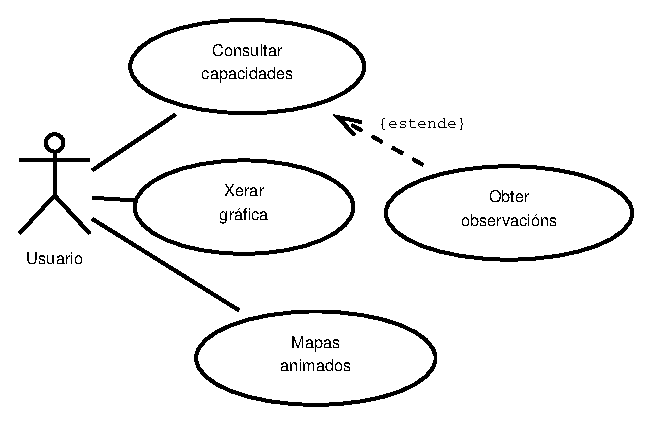
\includegraphics[width=0.8\textwidth]{images/uc.eps}
\caption{Diagrama de casos de uso}
\label{fig:uc} 
\end{figure}

\section{Catálogo de requisitos}
A partir dos casos de uso documentados realizase a extracción dos requisitos da aplicación. Estes requisitos son as características que debe presentar a aplicación, e definen o software desde o punto de vista do cliente. Dividimos os catálogo de requisitos en dúas partes, segundo a natureza dos mesmos:
\begin{description}
\item[Funcionais:] Son as características da aplicación para proporcionar a funcionalidade requirida.
\item[Non funcionais:] Non describen funcionalidades, se non que representan outras necesidades como seguridade, rendemento, usabilidade, ou restricións de plataforma, tecnolóxicas, e similares.
\end{description}

Clasificaremos os requisitos pola súa relevancia segundo o cadro \ref{tab:relevanciaReq}, que se terá en conta na planificación dos sprints.
\begin{table}
\begin{tabularx}{\textwidth}{lX} \toprule
	Relevancia & Descrición \\
	\midrule
	Esixido & Requisito que está directamente relacionado co cumprimento dos obxectivos do proxecto.\\
	Desexado & Requisito que mellora a calidade do proxecto, pero non está relacionado directamente cos obxectivos do mesmo.\\
	Opcional &  Requisito que non supón unha mellora substancial na calidade do proxecto, aínda que si resulta de utilidade.\\
	\bottomrule
\end{tabularx}
\caption{Niveis de relevancia dun requisito}
\label{tab:relevanciaReq}
\end{table}

\subsection{Requisitos funcionais}
Os requisitos funcionais definidos, verificados e revisados para o presente proxecto son os que seguen:

\reqtable 	{RF.01}{Conectar con servidor SOS}
		  	{O usuario pode introducir o enderezo dun servidor que proporcione o servizo SOS e obter do mesmo as súas capacidades. Estas capacidades deben visualizarse nun formato amigable para o usuario.}%Descrición
			{Esixido}%Relevancia
			{O requisito cumprirase se a aplicación e capaz de conectarse cos servidores indicados e procesar o resultado da operación \emph{GetCapabilities} para visualizala nun formato lexible.}%Criterio de validación
			
\reqtable 	{RF.02}{Gardar lista de servidores SOS}
		  	{O usuario poderá xestionar unha lista de servidores SOS para os que se indicará o enderezo e un nome para identificalo.}%Descrición
			{Opcional}%Relevancia
			{O requisito cumprirase se a aplicación permite gardar unha lista de servidores e facer o mantemento da mesma.}%Criterio de validación
			
\reqtable 	{RF.03}{Visualizar XML das capacidades do servidor}
		  	{O usuario poderá visualizar en formato texto, con resaltado de sintaxe, e nun visor de árbore o XML que describe as capacidades do servidor.}%Descrición
			{Desexado}%Relevancia
			{O requisito cumprirase se a aplicación dispón dun visor de XML con resaltado de sintaxe e visor de árbore no que se amose o ficheiro resposta do servidor á petición \emph{GetCapabilities}.}%Criterio de validación
			
\reqtable 	{RF.04}{Xerar capa vectorial cas observacións do servidor}
		  	{Unha vez consultadas as capacidades do servidor, o usuario poderá seleccionar unha oferta e unha ou varias das propiedades da mesma para descargar os datos e xerar unha capa vectorial coas observacións descargadas.}%Descrición
			{Esixido}%Relevancia
			{O requisito cumprirase se a aplicación descarga os datos solicitados do servidor e os procesa XML creando un rexistro na capa vectorial para cada observación, cos datos de xeometría, tempo e o valor de cada propiedade.}%Criterio de validación
			
\reqtable 	{RF.05}{Permitir filtrado básico das observacións a descargar}
		  	{O usuario poderá indicar o rango de tempo no que lle interesan as observacións, así como un ou máis sensores e unha ou máis entidades.}%Descrición
			{Esixido}%Relevancia
			{O requisito cumprirase se a través de interface se pode seleccionar un rango de tempo, unha lista de sensores e unha lista de entidades e estes datos se inclúen no XML para a operación \emph{GetObservations}.}%Criterio de validación
\newpage			
\reqtable 	{RF.06}{Permitir filtrado avanzado das observacións a descargar}
		  	{O usuario poderá indicar un filtro espacial que delimite a zona da que quere obter as observacións. A interface mostrará os operadores e tipos de operandos soportados polo servizo. Tamén se poderá indicar un filtro escalar por algunha das propiedades da oferta seleccionada. A interface so mostrará os operandos soportados polo servizo.}%Descrición
			{Desexado}%Relevancia
			{O requisito cumprirase se a través de interface se pode indicar un filtro espacial, seleccionando a xeometría sobre o mapa, e un filtro escalar para algunha das propiedades observadas e estes datos se inclúen no XML para a operación \emph{GetObservations}.}%Criterio de validación
			
\reqtable 	{RF.07}{Xerar petición de observacións manualmente}
		  	{O usuario poderá modificar en modo texto o XML xerado a través da interface gráfica,  para obter as observacións desexadas.}%Descrición
			{Opcional}%Relevancia
			{O requisito cumprirase se a aplicación permite visualizar e modificar o XML a usar para a operación \emph{GetObservations}.}%Criterio de validación
			
\reqtable 	{RF.08}{Xerar gráfica propiedade \emph{vs} tempo}
		  	{O usuario poderá, a partir dunha entidade seleccionada no mapa, visualizar unha gráfica que mostre unha liña coa evolución temporal da propiedade observada.}%Descrición
			{Esixido}%Relevancia
			{O requisito cumprirase se a aplicación mostra unha gráfica de liña representando o tempo no eixo X e os valores da propiedade observada no eixo Y.}%Criterio de validación
			
\reqtable 	{RF.09}{Xerar gráfica para enfrontar dúas propiedades}
		  	{O usuario poderá, a partir dunha entidade seleccionada no mapa, visualizar unha gráfica de puntos indicando unha propiedade para o eixo X e outra para o Y.}%Descrición
			{Desexado}%Relevancia
			{O requisito cumprirase se a aplicación}%Criterio de validación
			
\reqtable 	{RF.10}{Xerar gráfica con varias series}
		  	{O usuario poderá seleccionar varias entidades no mapa, e cada unha delas será unha serie de datos na gráfica visualizada. O usuario poderá configurar o estilo de cada unha das series.}%Descrición
			{Desexado}%Relevancia
			{O requisito cumprirase se a aplicación permite xerar gráficas con varias entidades seleccionadas, de xeito que as observacións de cada entidade teñan un formato diferente. O tipo de liña, de marcador, e a cor de cada serie de datos ten que poder modificarse.}%Criterio de validación
			
\reqtable 	{RF.11}{Xerar animación no visor de mapas}
		  	{O usuario disporá dunha barra de tempo integrada no visor de mapas, que permitirá visualizar só as observacións correspondentes o tempo indicado nesta barra. Ademais disporá dun botón de reprodución que desprazará esta barra automaticamente.}%Descrición
			{Opcional}%Relevancia
			{O requisito cumprirase se a aplicación xera unha capa válida para ser engadida ó \emph{plugin} TimeManager de QGIS.}%Criterio de validación

\subsection{Requisitos non funcionais}
Os requisitos non funcionais definidos, verificados e revisados para o presente proxecto son os que seguen:

\reqtable 	{RNF.01}{Versión de SOS 1.0}
		  	{A pesar de existir a versión 2.0 do estándar SOS debe soportarse a versión 1.0, pois esta é a que implementan os servidores desenvolvidos polo CiTIUS.}%Descrición
			{Esixido}%Relevancia
			{O requisito cumprirase se a aplicación é capaz de comunicarse con servidores que implementen a versión 1.0 do estándar SOS.}%Criterio de validación
			
\reqtable 	{RNF.02}{Linguaxe de programación Python}
		  	{QGIS soporta \emph{plugins} programados en C++ ou en Python, pero so os programados en Python son instalables desde o xestor de \emph{plugins} incorporado na aplicación.}%Descrición
			{Desexado}%Relevancia
			{A aplicación programarase en linguaxe Python.}%Criterio de validación
			
\reqtable 	{RNF.03}{Consistencia da interface gráfica}
		  	{Dado que a aplicación a desenvolver é un \emph{plugin} que se integrará dentro da propia aplicación QGIS o aspecto e deseño da interface gráfica debe ser consistente coa do propio QGIS.}%Descrición
			{Desexado}%Relevancia
			{O requisito cumprirase se usuarios habituados ó QGIS son capaces de usar o \emph{plugin} sin necesidade de indicacións.}%Criterio de validación

\reqtable 	{RNF.04}{Manual de usuario}
		  	{O usuario terá a súa disposición un manual de uso da aplicación.}%Descrición
			{Esixido}%Relevancia
			{O requisito cumprirase se a memoria do proxecto inclúe un apéndice no que se explique o funcionamento básico do \emph{plugin}.}%Criterio de validación
			
\reqtable 	{RNF.05}{Internacionalización da aplicación}
		  	{A aplicación deberá ser deseñada de xeito que poida ser adaptada para outras linguas sen a necesidade de facer cambios a nivel de código.}%Descrición
			{Opcional}%Relevancia
			{O requisito cumprirase se o \emph{plugin} pode ser traducido a distintos idiomas sen modificar o código fonte.}%Criterio de validación
			
\reqtable 	{RNF.06}{Data límite de execución do proxecto}
		  	{A data límite de entrega da documentación do proxecto é o venres 10 de Xullo de 2015, segundo o publicado na páxina web da Escola Técnica Superior de Enxeñaría\footnote{\url{http://www.usc.es/etse/files/u1/datasdefensa14_15GREI.pdf}}.}%Descrición
			{Esixido}%Relevancia
			{-}%Criterio de validación

\section{Matriz de trazabilidade}
A matriz de trazabilidade relaciona cada requisito co seu caso de uso de orixe. A matriz de trazabilidade para este proxecto é a representada no cadro \ref{tab:trazaRequisitos}.

\begin{table}[htbp]
\centering
\begin{tabular}{l|c|c|c|c|c|c|c|c|c|c|c|}
 & \rotatebox{90}{\ref{req:RF.01}} & \rotatebox{90}{\ref{req:RF.02}} & \rotatebox{90}{\ref{req:RF.03}} & \rotatebox{90}{\ref{req:RF.04}} & \rotatebox{90}{\ref{req:RF.05}} & \rotatebox{90}{\ref{req:RF.06}} & \rotatebox{90}{\ref{req:RF.07}} & \rotatebox{90}{\ref{req:RF.08}} & \rotatebox{90}{\ref{req:RF.09}} & \rotatebox{90}{\ref{req:RF.10}} & \rotatebox{90}{\ref{req:RF.11}} \\ \hline
\ref{uc:CU.01} & $\bullet$ & $\bullet$ & $\bullet$ &  &  &  &  &  &  &  &  \\ \hline
\ref{uc:CU.02} &  &  &  & $\bullet$ & $\bullet$ & $\bullet$ & $\bullet$ &  &  &  &  \\ \hline
\ref{uc:CU.03} &  &  &  &  &  &  &  & $\bullet$ & $\bullet$ & $\bullet$ &  \\ \hline
\ref{uc:CU.04} &  &  &  &  &  &  &  &  &  &  & $\bullet$ \\ \hline
\end{tabular}
\caption{Matriz de trazabilidade de requisitos}
\label{tab:trazaRequisitos}
\end{table}\cleardoublepage
\chapter{Deseño do software}
Neste capítulo descríbese a arquitectura do sistema a desenvolver desde un punto de vista global, identificando as distintas compoñentes que o conforman e a forma de relacionarse entre elas, tanto dende o punto de vista estrutural como desde o punto te vista interacción entre elas.

\section{Arquitectura do sistema}
Dende a definición dos obxectivos do proxecto identifícanse dúas partes diferenciadas dentro do sistema a desenvolver. Por un lado a comunicación co servidor SOS, para a obtención das súas capacidades e dos datos de observacións, e por outro a visualización e explotación das observacións descargadas. Esta división trasladase directamente á estrutura da aplicación, que se amosa na figura \ref{fig:diaComponentes}, na que tamén se inclúen os compoñentes externos cos que se relacionan.

\begin{figure}[hbtp]
 \centering
 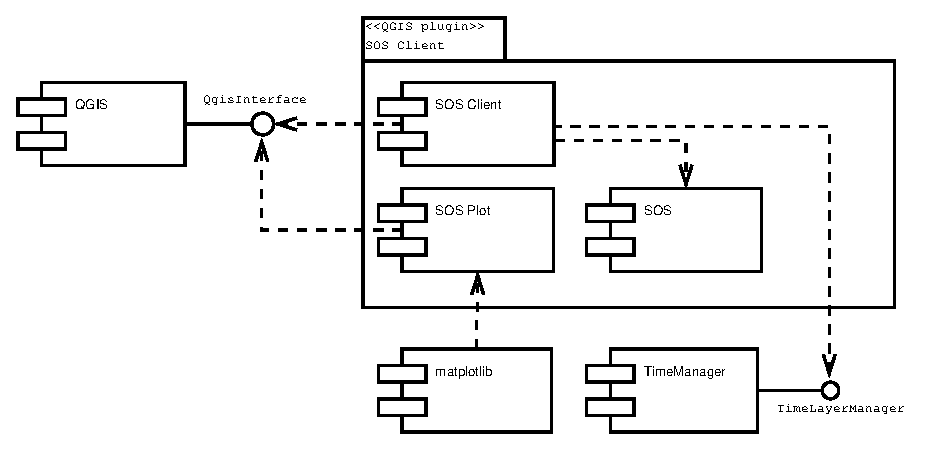
\includegraphics[width=0.5\textwidth]{images/componentes.eps}
 \caption{Diagrama de compoñentes}
 \label{fig:diaComponentes}
\end{figure}

A compoñente \textbf{SOS Client} é a responsable da comunicación co servidor SOS tanto a hora de xerar as peticións necesarias a partir da información proporcionada polo usuario e como para almacenar e interpretar as respostas do servizo.

A compoñente \textbf{SOS Plot} é a responsable de, a partir da capa vectorial xerada, visualizar as observacións segundo as preferencias indicadas polo usuario.

As compoñentes externas incluídas no diagrama son:
\begin{itemize}
\item QGIS: Representa á aplicación na que se integra o \emph{plugin}.
\item TimeManager\footnote{\url{https://plugins.qgis.org/plugins/timemanager/}}: É un \emph{plugin} para QGIS que engade controles de tempo o mesmo, de xeito que se podan animar as capas vectoriais directamente no visor de mapas, en base a un atributo de tempo.
\item matplotlib\footnote{\url{http://matplotlib.org/}}: É unha librería de Python para debuxar gráficos en 2D que permite producir figuras de alta calidade, tanto para publicacións como en entornos interactivos.
\end{itemize}

\subsection{Patrón de arquitectura}
O uso dun patrón de arquitectura axeitado para o sistema a desenvolver facilita os procesos de implementación e probas, ó proporcionar un esquema de organización estrutural dividindo o sistema en partes segundo a súa responsabilidade.

Os patróns de arquitectura máis amplamente utilizados no desenvolvemento de aplicacións son o MVC (\emph{Model-View-Controller}) e os seus derivados. O obxectivo principal destes patróns é separar o modelo de datos, a súa visualización e a lóxica de negocio facilitando de xeito moi significativo o mantemento e evolución das aplicacións.

Dadas as características concretas desde desenvolvemento optouse por unha simplificación do patrón MVC combinando a lóxica de negocio coas vistas, dando lugar a unha arquitectura denominada \emph{Model/View}\footnote{\url{http://doc.qt.io/qt-4.8/model-view-programming.html}}. Os motivos principais para levar a cabo esta simplificación son:
\begin{itemize}
\item A lóxica de negocio da aplicación e moi sinxela.
\item As librerías para o desenvolvemento das vistas veñen impostas pola aplicación na que se integrará o \emph{plugin}. As propias librerías están deseñadas para facilitar este patrón.
\end{itemize}

É importante destacar que aínda que se se incorpore a lóxica de negocio nas vistas, si que se mantén a separación entre a creación e configuración dos compoñentes gráficos do resto de lóxica da vista. A creación dos compoñentes gráficos faise a través dunha factoría que os xera directamente desde a súa definición XML.

Na figura \ref{fig:MVCvsMV} móstrase de xeito gráfico a diferencia entre o patrón MVC e o \emph{Model/View}. O \emph{Model/View}, amais da vista e o modelo, inclúe o concepto \emph{Delegate}, que representa a un mediador entre a vista e o modelo para facilitar a personalización de como se mostran e editan determinados datos.

\begin{figure}[hbtp]
 \centering
 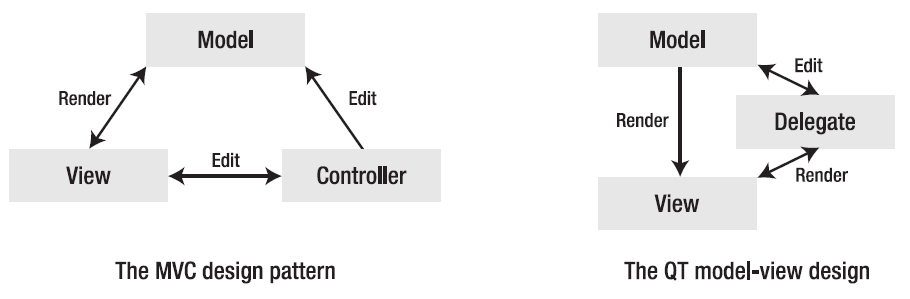
\includegraphics[width=\textwidth]{images/MVCvsMV.png}
 \caption{Diferencias entre MVC e Model/View}
 \label{fig:MVCvsMV}
\end{figure}

\section{Interacción entre compoñentes}
Para describir o comportamento do sistema desde un punto de vista dinámico empréganse os diagramas de secuencia, nos que se describe a interacción entre as distintas compoñentes do sistema para cumprir cada caso de uso definido.

Para conseguir un nivel de detalle suficiente para describir o comportamento do sistema dividisen as compoñentes segundo a arquitectura proposta. A compoñente SOSClient divídese en SOSClientDialog, que representa a vista, e Sensor Observation Service, que representa o modelo. No caso da compoñente SOSPlot, a vista é representada pola compoñente SOSPlotDialog e o modelo non se representa de xeito independente pois está incluído dentro da compoñente matplotlib.

No diagrama \ref{fig:diaSeq1-2} inclúense os caso de uso \ref{uc:CU.01} e \ref{uc:CU.02}, xa que o \ref{uc:CU.02} estende ó \ref{uc:CU.01}, polo que é máis claro representalos xuntos.
\begin{figure}
 \centering
 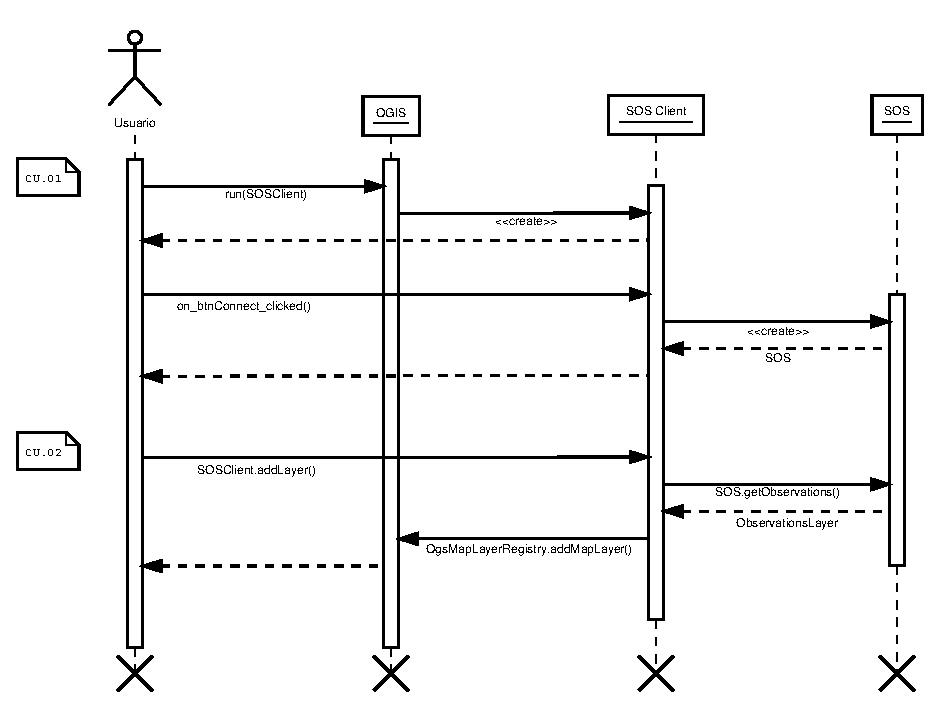
\includegraphics[width=\textwidth]{images/seq1-2.eps}
 \caption{Diagrama de secuencia para os casos de uso \ref{uc:CU.01} e \ref{uc:CU.02}}
 \label{fig:diaSeq1-2}
\end{figure}

O diagrama \ref{fig:diaSeq3} representa o comportamento para o caso de uso \ref{uc:CU.03}.
\begin{figure}
 \centering
 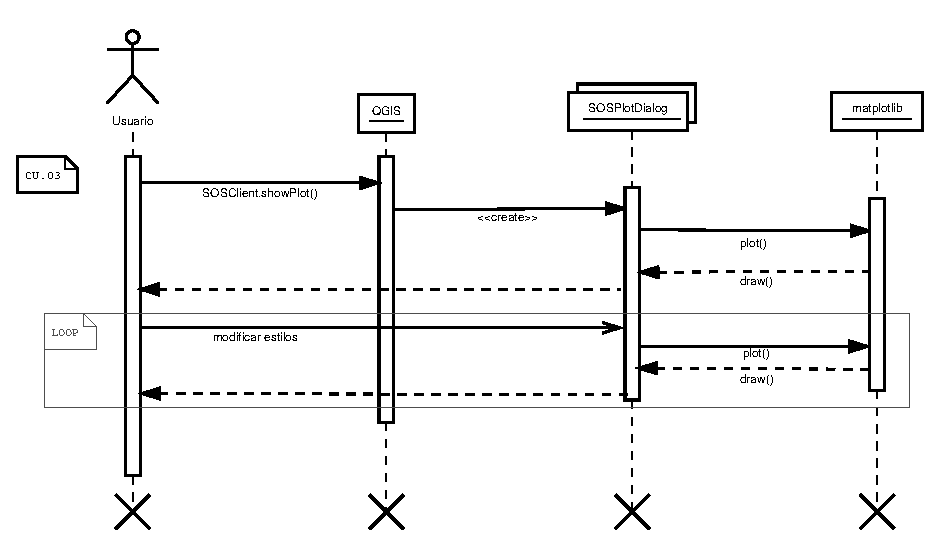
\includegraphics[width=\textwidth]{images/seq3.eps}
 \caption{Diagrama de secuencia para o caso de uso \ref{uc:CU.03}}
 \label{fig:diaSeq3}
\end{figure}

Para cubrir a funcionalidade requirida polo caso de uso \ref{uc:CU.04} existe o \emph{plugin} \emph{TimeManager} para QGIS, polo que o que representa o diagrama \ref{fig:diaSeq4} é o procedemento para que a capa xerada coas observacións sexa controlada polo \emph{TimeManager}.
\begin{figure}
 \centering
 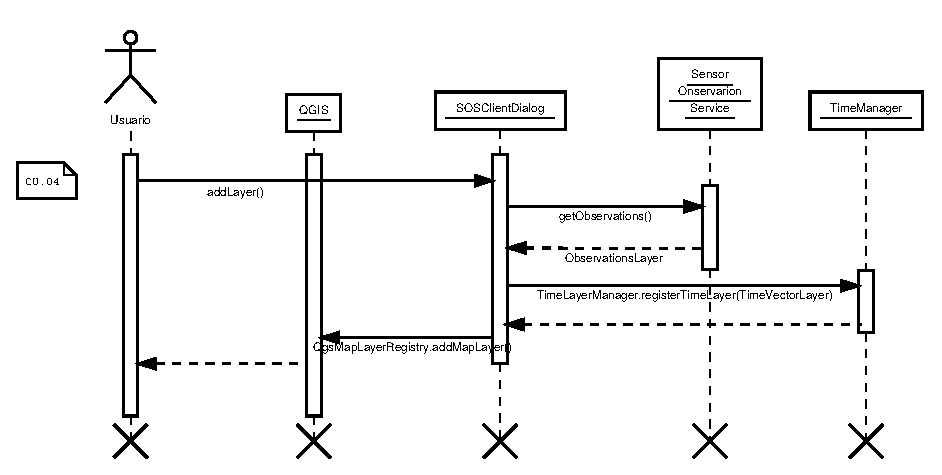
\includegraphics[width=\textwidth]{images/seq4.eps}
 \caption{Diagrama de secuencia para o caso de uso \ref{uc:CU.04}}
 \label{fig:diaSeq4}
\end{figure}\cleardoublepage
\chapter{Desenvolvemento dos sprints}

A implementación deste proxecto consta de tres ciclos de sprint nos que se desenvolven as dúas compoñentes nas que está dividido. Cada un dos sprints consta das fase de análise, deseño, implementación e probas. Dado que a análise se describiu por completo no capítulo 2, neste capítulo detallaranse o deseño, implementación e probas realizadas para validar os requisitos planificados en cada un dos sprints.

A previsión inicial do contido de cada sprint está recollida no cadro \ref{tab:previsionSprints}, no capítulo de Xestión do proxecto. Neste apartado describirase xa a pila de cada sprint en base ós requisitos definidos, é dicir, o resultado da planificación do sprint. Cabe destacar que para a planificación do sprint non so se ten en conta a relevancia asignada a cada requisito, se non tamén o tempo estimado para levalo a cabo e a súa repercusión no cumprimento dos requisitos non funcionais.

\section{Sprint 1}
Os requisitos funcionais que se inclúen na pila do primeiro sprint son:
\begin{itemize}
\item \ref{req:RF.01}.- Conectar con servidor SOS
\item \ref{req:RF.02}.- Gardar lista de servidores SOS
\item \ref{req:RF.04}.- Xerar capa vectorial cas observacións do servidor
\end{itemize}

Neste ciclo de desenvolvemento levouse a cabo o deseño inicial da interface gráfica para a ventá de conexión co servidor SOS, seguindo como guía as ventás dispoñibles de xeito nativo no QGIS para descargar datos de outros servizos similares (WFS, WMS, WCS), co obxectivo de satisfacer o requisito \ref{req:RNF.03}.

Outra tarefa importante levada a cabo foi a definición dunha estrutura extensible para o módulo de procesamento do XML, de xeito que sexa sinxelo engadir as distintas casuísticas que vaian aparecendo, debido a gran liberdade que dan os estándares SOS e O\&M. Tamén se analizaron distintas posibilidades para o procesamento do XML en Python, sendo todas elas moi similares en canto a funcionalidade, optouse por empregar o módulo para XML das propias librerías Qt para non engadir dependencias innecesarias.

No diagrama \ref{fig:diaClassSOSClient} represéntanse o deseño de clases realizado, que se corresponde coa compoñente SOSClient. Móstranse so os atributos e métodos máis relevantes para entender a función de cada clase, que se representan separadas entre vista e modelo. Agrupadas sobre fondo escuro represéntanse as clases encargadas do procesamento dos documentos XML proporcionados polo servizo SOS.

\begin{sidewaysfigure}
 \centering
 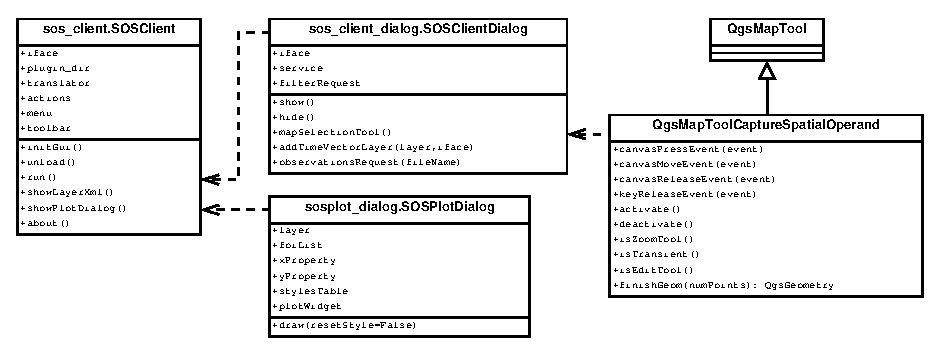
\includegraphics[width=\textwidth]{images/clases_sos_client.eps}
 \caption{Diagrama de clases da compoñente SOS Client}
 \label{fig:diaClassSOSClient}
\end{sidewaysfigure}

As clases máis relevantes da figura \ref{fig:diaClassSOSClient} son:
\begin{description}
\item[WidgetFactory:] É unha factoría de clases que crea, a partir dos XML de definición da interface, as clases cos compoñentes gráficos. A implementación real da vista farase en clases que herdarán da clase correspondente creada por esta factoría.
\item[SOSClientDialog:] É o formulario xeral de comunicación cos servidores SOS. Contén a lóxica de funcionamento da vista e as chamadas necesarias ás clases que forman o modelo.
\item[SensorObservationService:] Esta clase representa o servizo SOS. Créase a partir do XML que define as capacidades do servizo e almacena toda a información necesaria para que a vista poda presentar o usuario as opcións correspondentes para xerar as consultas.
\item[ObservationsLayer:] Esta clase é a encargada de construír a capa vectorial para o QGIS, a partir da clase SOSProvider.
\item[SOSProvider:] Simula unha clase QgsVectorDataProvider\footnote{\url{http://qgis.org/api/classQgsVectorDataProvider.html}}. É pois a clase que fai de intermediaria entre a estrutura de datos real da información da capa e a estrutura manexada polo QGIS.
\item[XMLParserFactory:] É unha factoría para crear as distintas clases para o procesamento dos XML. A partir da etiqueta XML atopada devolve a clase encargada de procesar o nodo.
\item[XMLParser:] Clase base para todas as clases de procesamento de XML.
\end{description}

Tamén se preparou durante este sprint o entorno para a automatización das probas unitarias a través da ferramenta \emph{PyUnit}\footnote{\url{https://docs.python.org/2/library/unittest.html}} e programáronse varios casos de probas para o módulo de procesamento de XML en base a ficheiros de exemplo.

Co obxectivo de validar o incremento xerado leváronse a cabo as seguintes probas:

\testtable{PR.01}{Conexión con servidor SOS}
		  {\begin{itemize}\item \ref{req:RF.01} \item \ref{req:RNF.03}\end{itemize}} %Requerimentos
		  {Compróbase, a parte das probas unitarias automáticas, a conexión con varios servidores SOS.} %Descripción
		  {\begin{itemize}
		  \item A información das capacidades do servizo visualízanse en formato HTML cos estilos propios de QGIS.
		  \item As ofertas dispoñibles visualízanse nunha caixa de selección, e as propiedades e procedementos relacionados en sendas listas nas que se poden marcar e desmarcar. Estas listas actualízanse correctamente ó modificar a oferta seleccionada.
		  \end{itemize}} %Resultado
		  
\testtable{PR.02}{Xestión de servidores}
		  {\begin{itemize}\item \ref{req:RF.02} \item \ref{req:RNF.03}\end{itemize}} %Requerimentos
		  {Próbanse as funcionalidades de alta, baixa e modificación de conexións na interface gráfica, así coma o correcto gardado entre distintas execucións da aplicación QGIS.} %Descripción
		  {Todas as operacións funcionan correctamente.} %Resultado

\testtable{PR.03}{Descargar observacións}
		  {\begin{itemize}\item \ref{req:RF.04} \\\end{itemize}} %Requerimentos
		  {Compróbase a execución da operación \emph{GetObservations} contra varios servidores.} %Descripción
		  {\begin{itemize}
		  \item O XML descárgase correctamente.
		  \item O XML procesase e obtéñense as xeometrías contidas no mesmo coas que se crea unha capa vectorial en memoria no QGIS.
		  \end{itemize}} %Resultado
		  
O \ref{req:RF.04} cubriuse parcialmente, pois aínda que se podían visualizar no mapa os puntos correspondentes as observacións o resto de información do XML se trata correctamente.

Tendo en conta a matriz de trazabilidade do cadro \ref{tab:trazaRequisitos}, este primeiro incremento non resolve ningún caso de uso completo.

\section{Sprint 2}
Na pila do segundo sprint inclúense os seguintes requisitos funcionais:
\begin{itemize}
\item \ref{req:RF.04}.- Xerar capa vectorial cas observacións do servidor (continuación)
\item \ref{req:RF.03}.- Visualizar XML das capacidades do servidor
\item \ref{req:RF.05}.- Permitir filtrado básico das observacións a descargar
\item \ref{req:RF.07}.- Xerar petición de observacións manualmente
\item \ref{req:RF.11}.- Xerar animación no visor de mapas
\item \ref{req:RF.08}.- Xerar gráfica propiedade vs tempo
\end{itemize}

No segundo ciclo de sprint conclúese o módulo de procesamento XML para interpretar correctamente todos os datos das observacións resultado da operación \emph{GetObservations}, tanto co modelo \emph{Observations} como co \emph{Measurements}. Amais comprobase que requisitos debe cumprir a capa para poder ser xestionada a través do plugin \emph{TimeManager}, e impleméntase o proceso de creación da capa tendo en conta estes requisitos.

Tamén se implementan os filtros básicos de observacións, e por ser de utilidade para o proceso de desenvolvemento e probas tamén se implementa a visualización do XML das capacidades do servidor e a posibilidade de visualizar e editar o XML xerado para a petición de observacións.

En canto a xeración de gráficas realízanse varias probas coa librería matplotlib.

Co obxectivo de validar o incremento xerado leváronse a cabo as seguintes probas:

\testtable{PR.04}{Procesamento de XML con observacións en formato \emph{Observations} e \emph{Measurements}}
		  {\begin{itemize}\item \ref{req:RF.04} \\\end{itemize}} %Requerimentos
		  {Codifícanse probas unitarias para a validación do módulo de procesamento so XML de observacións nos dous formatos, en base a ficheiros de exemplos dos servidores SOS do CiTIUS.} %Descripción
		  {\begin{itemize}
		  \item O XML procesase correctamente, detectando os campos de tipo tempo, os numéricos e as cadeas de texto.
		  \item A partir da estrutura de datos xerada a partir do XML crease correctamente unha capa vectorial no QGIS, con todos os campos contidos na observación e cos valores correctos.
		  \end{itemize}} %Resultado

\testtable{PR.05}{Xeración de filtros para \emph{GetObservations}}
		  {\begin{itemize}\item \ref{req:RF.03} \item \ref{req:RF.05} \item \ref{req:RF.07}\end{itemize}} %Requerimentos
		  {Comprobar que os obxectos de interface conteñen os valores correctos segundo as capacidades do SOS e que o XML que se xera a través das distintas opcións de interface é válido.} %Descripción
		  {\begin{itemize}
		  \item Comprobase conectando con varios servidores que as opcións habilitadas nas distintas lapelas de filtros se corresponden coas capacidades definidas no XML.
		  \item A lista de sensores seleccionados e a de entidades de interese, así como o operador e operandos dos filtros de tempo inclúense correctamente no XML para a petición \emph{GetObservations}.
		  \end{itemize}} %Resultado

\testtable{PR.06}{Xestionar capa co \emph{TimeManager}}
		  {\begin{itemize}\item \ref{req:RF.04} \item \ref{req:RF.11} \end{itemize}} %Requerimentos
		  {Comprobar o correcto funcionamento do plugin \emph{TimeManager} coa capa creada.} %Descripción
		  {\begin{itemize}
		  \item Comprobase que a capa se engade á lista das xestionadas polo \emph{TimeManager} de xeito satisfactorio.
		  \item Verificase que o campo de tempo se interpreta correctamente.
		  \item Comprobase o funcionamento xeral do \emph{TimeManager} con varias capas de observacións.
		  \end{itemize}} %Resultado
		  
\testtable{PR.07}{Gráfica tempo \emph{vs} propiedade}
		  {\begin{itemize}\item \ref{req:RF.08} \\\end{itemize}} %Requerimentos
		  {Xerar gráfica co tempo no eixo X e a propiedade no Y.} %Descripción
		  {\begin{itemize}
		  \item A gráfica contén todas as observacións co mesmo \emph{foi} que a entidade seleccionada no mapa.
		  \item As observacións ordénanse polo campo tempo de xeito que se poda trazar unha liña que as una.
		  \item Ós valores do eixo X dáselles formato de tempo.
		  \end{itemize}} %Resultado
		  
Tendo en conta a matriz de trazabilidade do cadro \ref{tab:trazaRequisitos}, con este segundo incremento cúbrense os casos de uso \ref{uc:CU.01} e \ref{uc:CU.04}.
		  
\section{Sprint 3}
Na pila do terceiro sprint inclúense os seguintes requisitos funcionais:
\begin{itemize}
\item \ref{req:RF.06}.- Permitir filtrado avanzado das observacións a descargar
\item \ref{req:RF.09}.- Xerar gráfica para enfrontar dúas propiedades
\item \ref{req:RF.10}.- Xerar gráfica con varias series
\end{itemize}

Neste incremento habilítase a ferramenta para introducir o filtro espacial seleccionando a xeometría directamente sobre o mapa, segundo o tipo de operando seleccionado.

Tamén se modifica a visualización de gráficas para permitir seleccionar as propiedades a visualizar, traballar con varias \emph{foi} seleccionadas e permitir modificar os estilos e textos da gráfica. Esta tarefa implica o deseño tanto da interface gráfica como da estrutura de clases da compoñente SOSPlot, que se representa no diagrama \ref{fig:diaClassSOSPlot}. Móstranse agrupadas todas as clases que cumpren co rol de \emph{Delegate}. As demais correspóndense coa vista, pois o modelo da compoñente SOSPlot está soportado por clases internas do QGIS (QgsVectorLayer) e de matplotlib (Line2D).

\begin{figure}
 \centering
 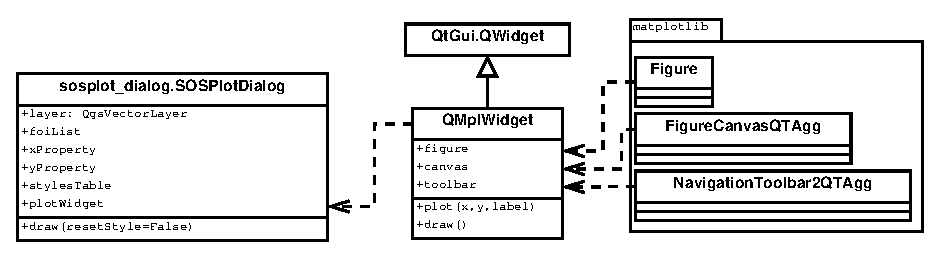
\includegraphics[width=\textwidth]{images/clases_sos_plot.eps}
 \caption{Diagrama de clases da compoñente SOS Plot}
 \label{fig:diaClassSOSPlot}
\end{figure}

As clases máis relevantes da figura \ref{fig:diaClassSOSPlot} son:
\begin{description}
\item[WidgetFactory:] Factoría para a xeración das compoñentes gráficas.
\item[SOSPlotDialog:] É o formulario de visualización de gráficos. Filtra e transforma os datos da capa vectorial activa para visualizalos no QMplWidget e conecta os distintos \emph{Delegates} co modelo.
\item[QMplWidget:] Clase que amalgama os obxectos da librería matplotlib para a visualización de gráficos.
\end{description}
\newpage
Co obxectivo de validar o incremento xerado leváronse a cabo as seguintes probas:

\testtable{PR.08}{Filtros espaciais}
		  {\begin{itemize}\item \ref{req:RF.06} \\\end{itemize}} %Requerimentos
		  {Comprobar o correcto funcionamento da ferramenta de selección de xeometrías e a inclusión no XML do filtro correspondente.} %Descripción
		  {\begin{itemize}
		  \item A ferramenta de selección permite debuxar rectángulos (indicando dous puntos), polígonos, liñas e puntos.
		  \item A xeometría debuxada no mapa transformase correctamente ó formato GML e inclúese no XML para a petición \emph{GetObservations}.
		  \end{itemize}} %Resultado
		  
\testtable{PR.09}{Xeración de gráficas con varias series}
		  {\begin{itemize}\item \ref{req:RF.10} \\\end{itemize}} %Requerimentos
		  {Compróbanse a xeración de gráficas a partir de varias entidades seleccionadas, de forma que cada \emph{foi} teña un estilo distinto.} %Descripción
		  {\begin{itemize}
		  \item Permítese xerar a gráfica con varias entidades seleccionadas. Para cada \emph{foi} distinto ordénanse os datos e debúxase a liña con unha cor distinta.
		  \item Permítese modificar a cor e estilo de cada liña e dos marcadores.
		  \end{itemize}} %Resultado
		  
\testtable{PR.10}{Personalización das propiedades das gráficas}
		  {\begin{itemize}\item \ref{req:RF.09} \\\end{itemize}} %Requerimentos
		  {Verificar que se poden modificar as distintas propiedades da gráfica, incluídas a propiedade a representar en cada eixo.} %Descripción
		  {\begin{itemize}
		  \item Pódense seleccionar o campo da capa a usar no eixo X e no eixo Y, así como por cal dos dous ordenar os datos para trazar liñas.
		  \item Permítese modificar os límites dos eixos X e Y manualmente.
		  \item Pódense modificar outras propiedades da gráfica como o título, as etiquetas e o formato de tempo.
		  \end{itemize}} %Resultado
		  
Tendo en conta a matriz de trazabilidade do cadro \ref{tab:trazaRequisitos}, con este terceiro incremento a aplicación permite levar a cabo os catro casos de uso definidos.\cleardoublepage
\chapter{Conclusións e posibles ampliacións}

Conclusións e posibles ampliacións
\cleardoublepage

% Aquí empezan os apéndices
\appendix
\chapter{Manual técnico}
TODO
Manuais técnicos: en función do tipo de Traballo e metodoloxía empregada, o contido poderase dividir en varios documentos. En todo caso, neles incluirase toda a información precisa para aquelas persoas que se vaian a encargar do desenvolvemento e/ou modificación do Sistema (por exemplo código fonte, recursos necesarios, operacións necesarias para modificacións e probas, posibles problemas, etc.). O código fonte poderase entregar en soporte informático en formatos PDF ou postscript.
\cleardoublepage
\chapter{Manual de usuario}
\section{Instalación}
O plugin pode instalarse desde a opción 'Administrar e instalar plugins' no menú Plugins do QGIS.
\begin{figure}[hbtp]
\centering
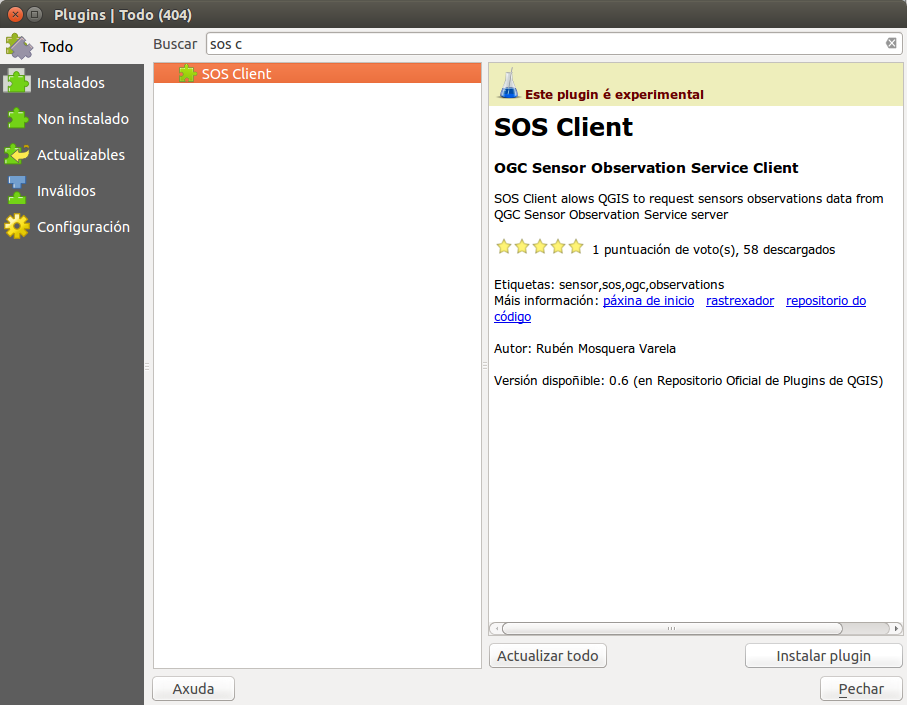
\includegraphics[width=0.8\textwidth]{images/manual/instalar.png}
\caption{Pantalla de instalación do plugin}
\label{fig:install}
\end{figure}

Unha vez instalado engadirase unha nova entrada no menú Web e tres novas accións na barra de ferramentas:
\begin{figure}[H]
\centering
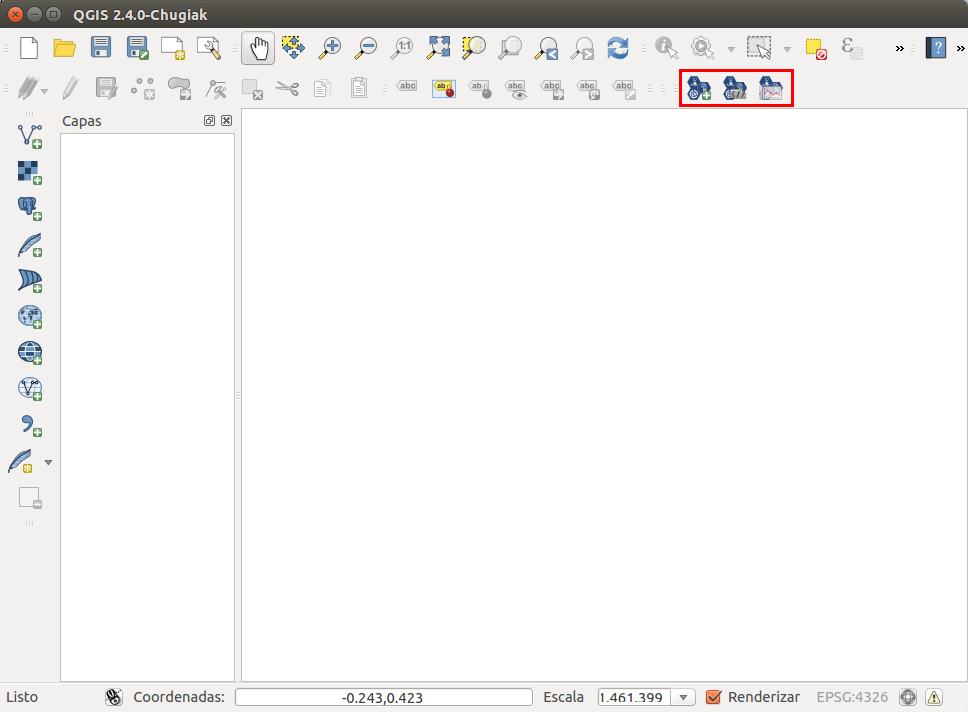
\includegraphics[width=0.8\textwidth]{images/manual/toolbar.png}
\caption{Barra de ferramentas do plugin}
\label{fig:toolbar}
\end{figure}

\begin{description}
\item [{
\includegraphics[width=24px]{images/manual/icon_add.png}}] Mostra o diálogo para conectar con un servidor SOS e engadir unha capa de observacións. 
\item [{
\includegraphics[width=24px]{images/manual/icon_xml.png}}] Visualiza o ficheiro XML usado para xerar a capa activa. 
\item [{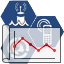
\includegraphics[width=24px]{images/manual/icon_plot.png}}] Xera unha gráfica coas observacións correspondentes ás entidades seleccionadas na capa activa.
\end{description}

\section{Crear capa de observacións}
Pulsando na acción 
\includegraphics[width=16px]{images/manual/icon_add.png} mostrase o formulario da figura \ref{fig:tabInfo-limpia}. Neste formulario pódese xestionar a lista de servidores cos botóns Novo, Editar e Eliminar, e co botón Conectar visualizar as capacidades do servidor seleccionado.
\begin{figure}[hbtp]
\centering
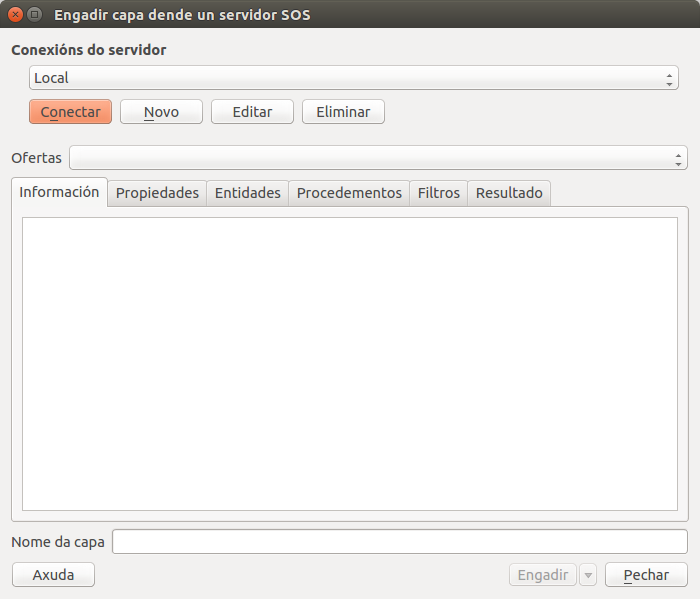
\includegraphics[width=0.8\textwidth]{images/manual/tabInfo-limpia.png}
\caption{Diálogo de conexión co servidor, sen datos}
\label{fig:tabInfo-limpia}
\end{figure}

Unha vez se conectou con un servidor móstranse as súas capacidades na lapela Información (figura \ref{fig:tabInfo}).
\begin{figure}[hbtp]
\centering
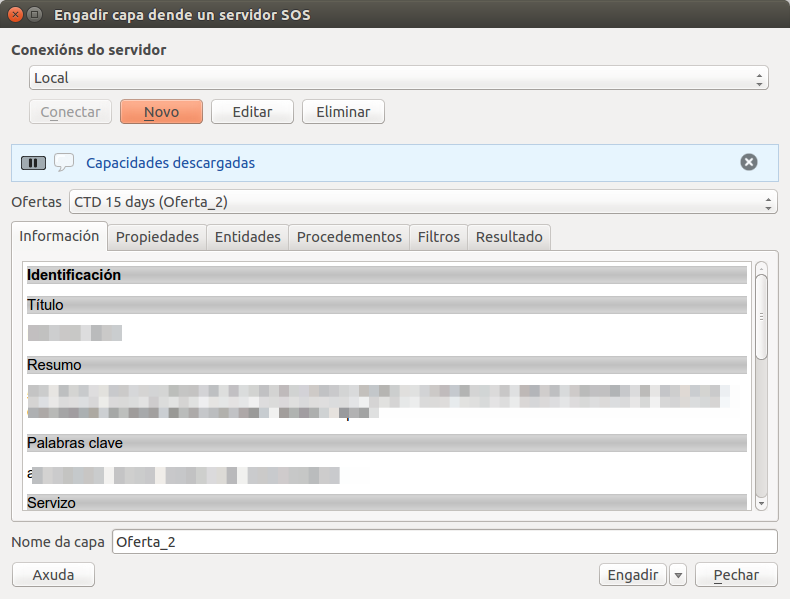
\includegraphics[width=0.8\textwidth]{images/manual/tabInfo.png}
\caption{Diálogo de conexión co servidor, con datos}
\label{fig:tabInfo}
\end{figure}

Para obter as observacións débese seleccionar unha oferta no campo Ofertas e pódese modificar o Nome da capa. As distintas lapelas do formulario descríbense no cadro \ref{tab:lapelas}:
\begin{table}[H]
\begin{tabularx}{\textwidth}{cX}
	\raisebox{-0.8\totalheight}{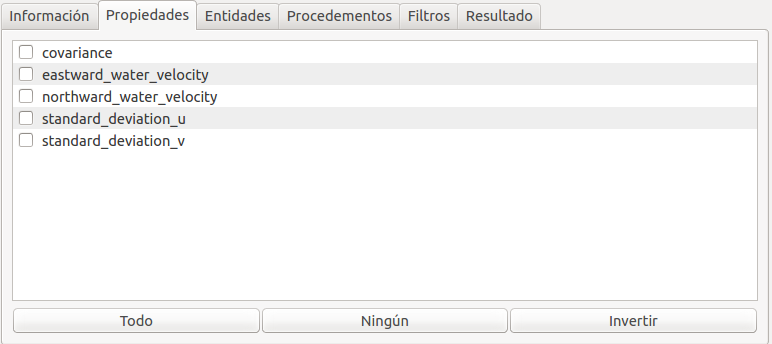
\includegraphics[width=0.4\textwidth]{images/manual/tabPropiedades.png}} & 
	Lista de propiedades da oferta. Pode seleccionar unha ou varias.\\
	\\
	\raisebox{-0.8\totalheight}{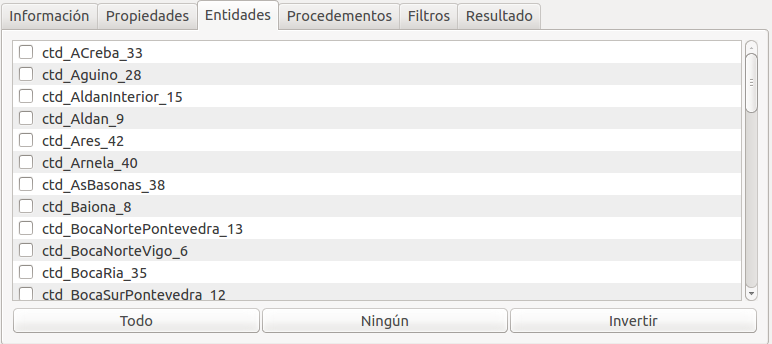
\includegraphics[width=0.4\textwidth]{images/manual/tabEntidades.png}} & Lista de entidades da oferta. Pode seleccionar varias ou ningunha.\\
	\\
	\raisebox{-0.8\totalheight}{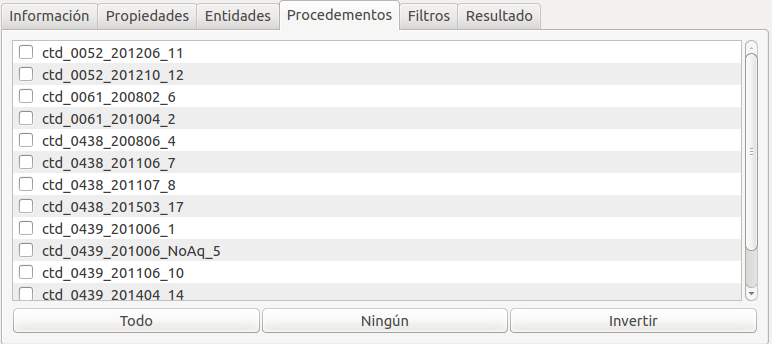
\includegraphics[width=0.4\textwidth]{images/manual/tabProcedementos.png}} & Lista de procedementos. Pode seleccionar varios ou ningún.\\
	\\
	\raisebox{-0.8\totalheight}{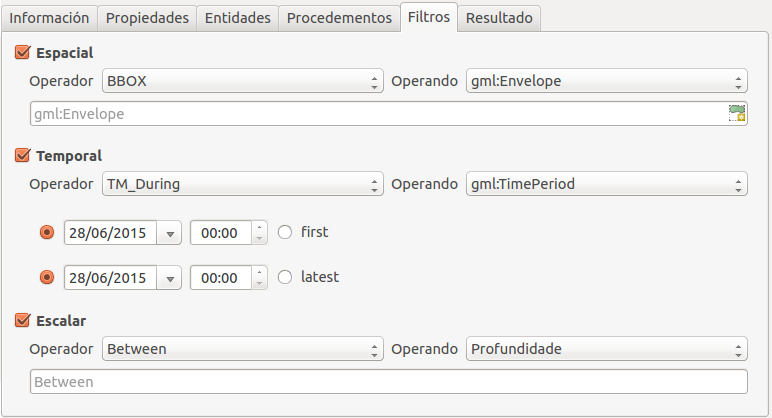
\includegraphics[width=0.4\textwidth]{images/manual/tabFiltros.png}} & Filtros dispoñibles. Pódense activar varios ó mesmo tempo. No caso do espacial, pulsando na icona poderase seleccionar a xeometría a consultar debuxando no mapa, como se amosa na figura \ref{fig:spatialtool}.\\
	\\
	\raisebox{-0.8\totalheight}{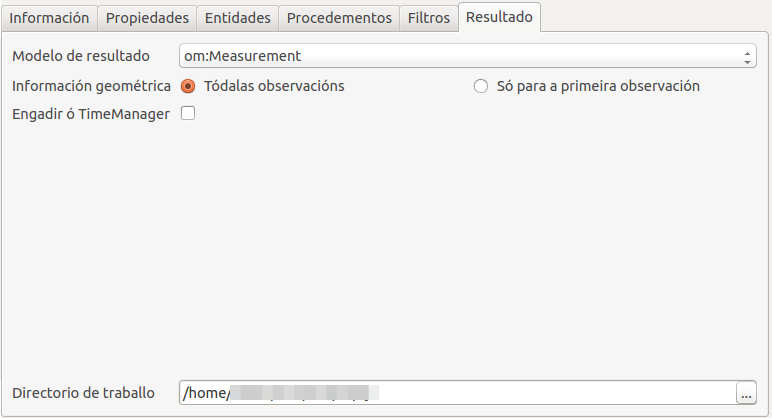
\includegraphics[width=0.4\textwidth]{images/manual/tabResultado.png}} & Pódese seleccionar o modelo de resultado entre os dispoñibles para o servidor. Permite indicar se todas as entidades terán información xeométrica ou so a primeira para cada \emph{foi} e seleccionar se engadir a capa ó TimeManager. Tamén se pode seleccionar o directorio de traballo no que se gardan os datos descargados.\\
\end{tabularx}
\caption{Lapelas do formulario de consulta ó SOS}
\label{tab:lapelas}
\end{table}

\begin{figure}[hbtp]
\centering
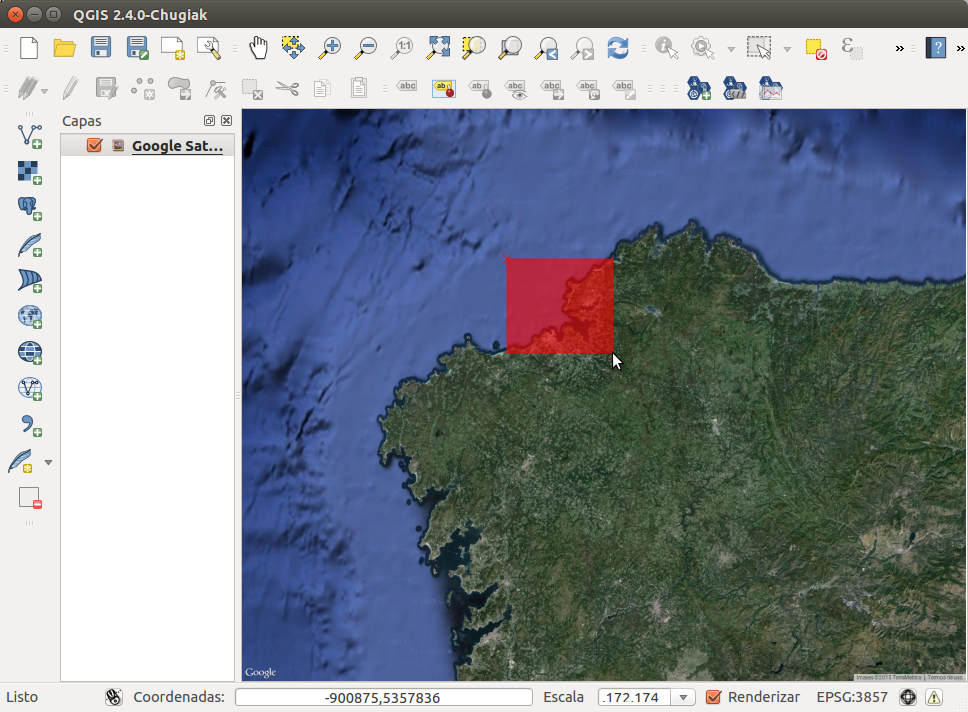
\includegraphics[width=0.8\textwidth]{images/manual/spatialtool.png}
\caption{Ferramenta de selección espacial}
\label{fig:spatialtool}
\end{figure}

Unha vez seleccionadas as opcións desexadas pódese engadir a capa ó QGIS pulsando no botón Engadir, ou cambiar o XML a enviar antes de engadir a capa co botón 'Editar petición', como se ve na figura \ref{fig:editarPeticion}.

\begin{figure}[hbtp]
\centering
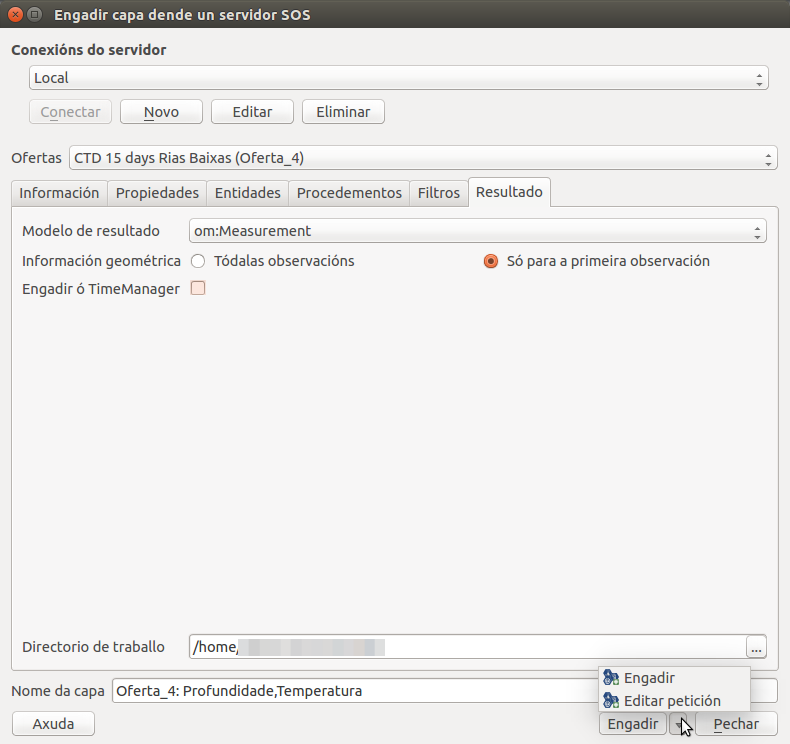
\includegraphics[width=0.8\textwidth]{images/manual/editar_peticion.png}
\caption{Engadir capa SOS}
\label{fig:editarPeticion}
\end{figure}

\section{Gráficos en dúas dimensións}

Para visualizar un gráfico é necesario que a capa activa teña unha ou máis entidades seleccionadas, e despois premer no botón 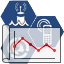
\includegraphics[width=16px]{images/manual/icon_plot.png}, como se amosa na figura \ref{fig:ejecutarSOSPlot}.

\begin{figure}[hbtp]
\centering
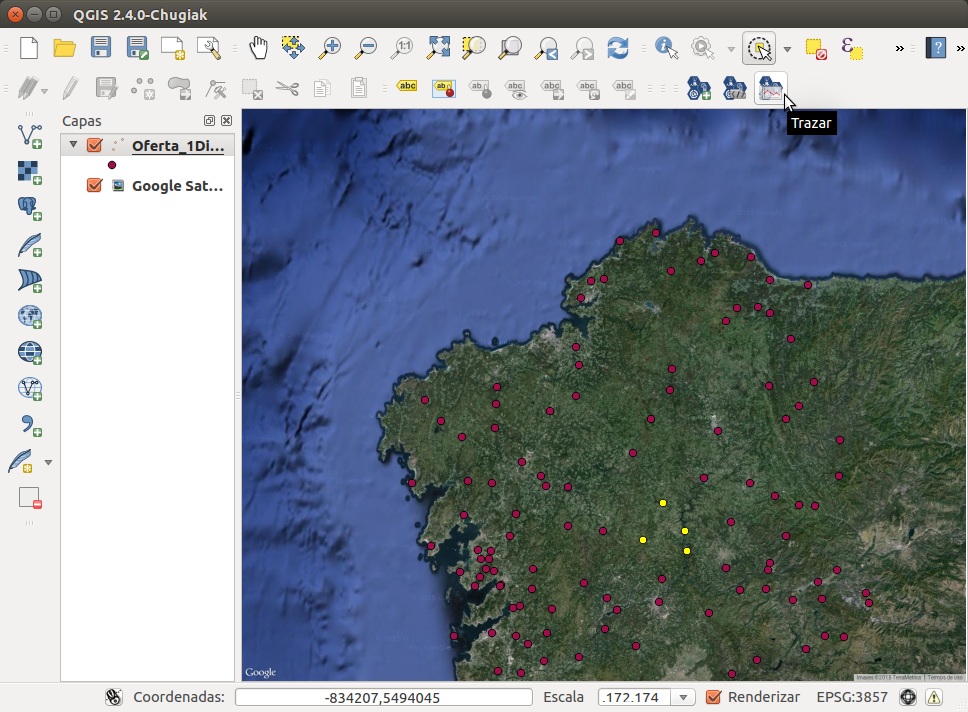
\includegraphics[width=\textwidth]{images/manual/ejecutar_sosplot.png}
\caption{Executar ferramenta SOS Plot}
\label{fig:ejecutarSOSPlot}
\end{figure}
\newpage
Esta operación abrirá unha nova ventá (figura \ref{fig:sosplot}) na que se visualizará a gráfica, e na que se poden editar as opcións do mesmo e interactuar coa gráfica.

\begin{figure}[hbtp]
\centering
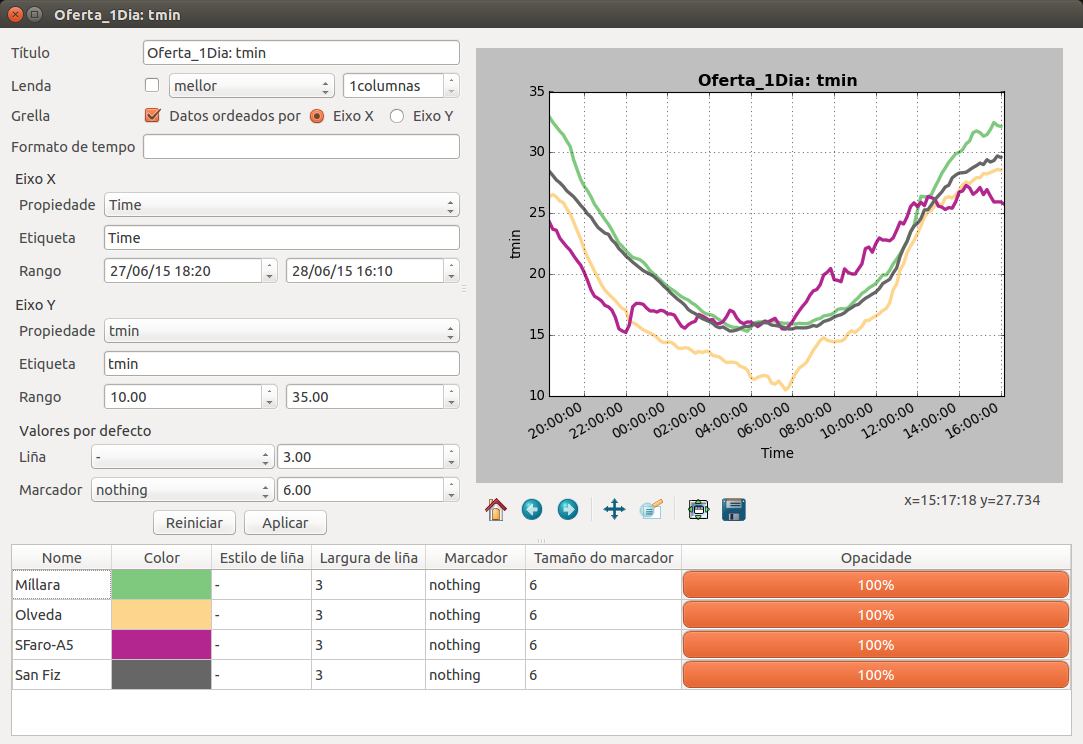
\includegraphics[width=\textwidth]{images/manual/sosplot.png}
\caption{SOS Plot: Gráfica de varias series}
\label{fig:sosplot}
\end{figure}

Neste formulario pódese editar o título do gráfico e dos eixos, a propiedade a representar en cada eixo e os límites dos mesmos, o formato no que representar o tempo, a inclusión dunha lenda, e o estilo e cor de liña e marcador de cada unha das series debuxadas. Amais sobre a gráfica pódese facer zoom, desprazala e gardar a imaxe.\cleardoublepage

\nocite{*}
\bibliography{bibliografia}
\bibliographystyle{plain}
\end{document}
